
% Emerging TFs
\section{Emerging Transcription Factors} \label{s:N_I:sel_tfs}

% Introduce the motivation of using TFs
After comparing the two community detection algorithm and deciding on the SBM, it is worth diving in the analysis of the network output. The previous sub-section showed that by prioritising a certain subset of genes, to have a higher minimum degree, has some effects on the network. However, in the network pipeline, not all the genes employed to generate the graph are used for the cancer stratification, but the top 100 selected by ModCon (see \cref{fig:N_I:network_pipeline}). The ModCon score is a score which takes in account a node's degree and their weights, thus well connected genes are selected.

% Presentin the Graph of sel TF-s. 
% -- all TF are included when minimum degree is set to 15 and there is no added benefit when TF = 6
\Cref{fig:N_I:sel_tfs} show the percentages of the TF genes (325 in total) that are selected by the ModCon score to stratify the disease. SBM community detection was used with both selected genes that are TF and non-TF 325 genes as control, the latter was run 10 times. It can be seen a clear difference between the Experiment and the Control traces, where the genes in the Experiment, with a real biological value, gradually increase with the minimum degree values. All the TF genes are included when the minimum degree of a TF reaches to 15 and the biggest percentage included after TF passes minimum degree of 6. Therefore, this value was chosen for selective edge pruning.


\begin{figure}[!b]   
    \centering
    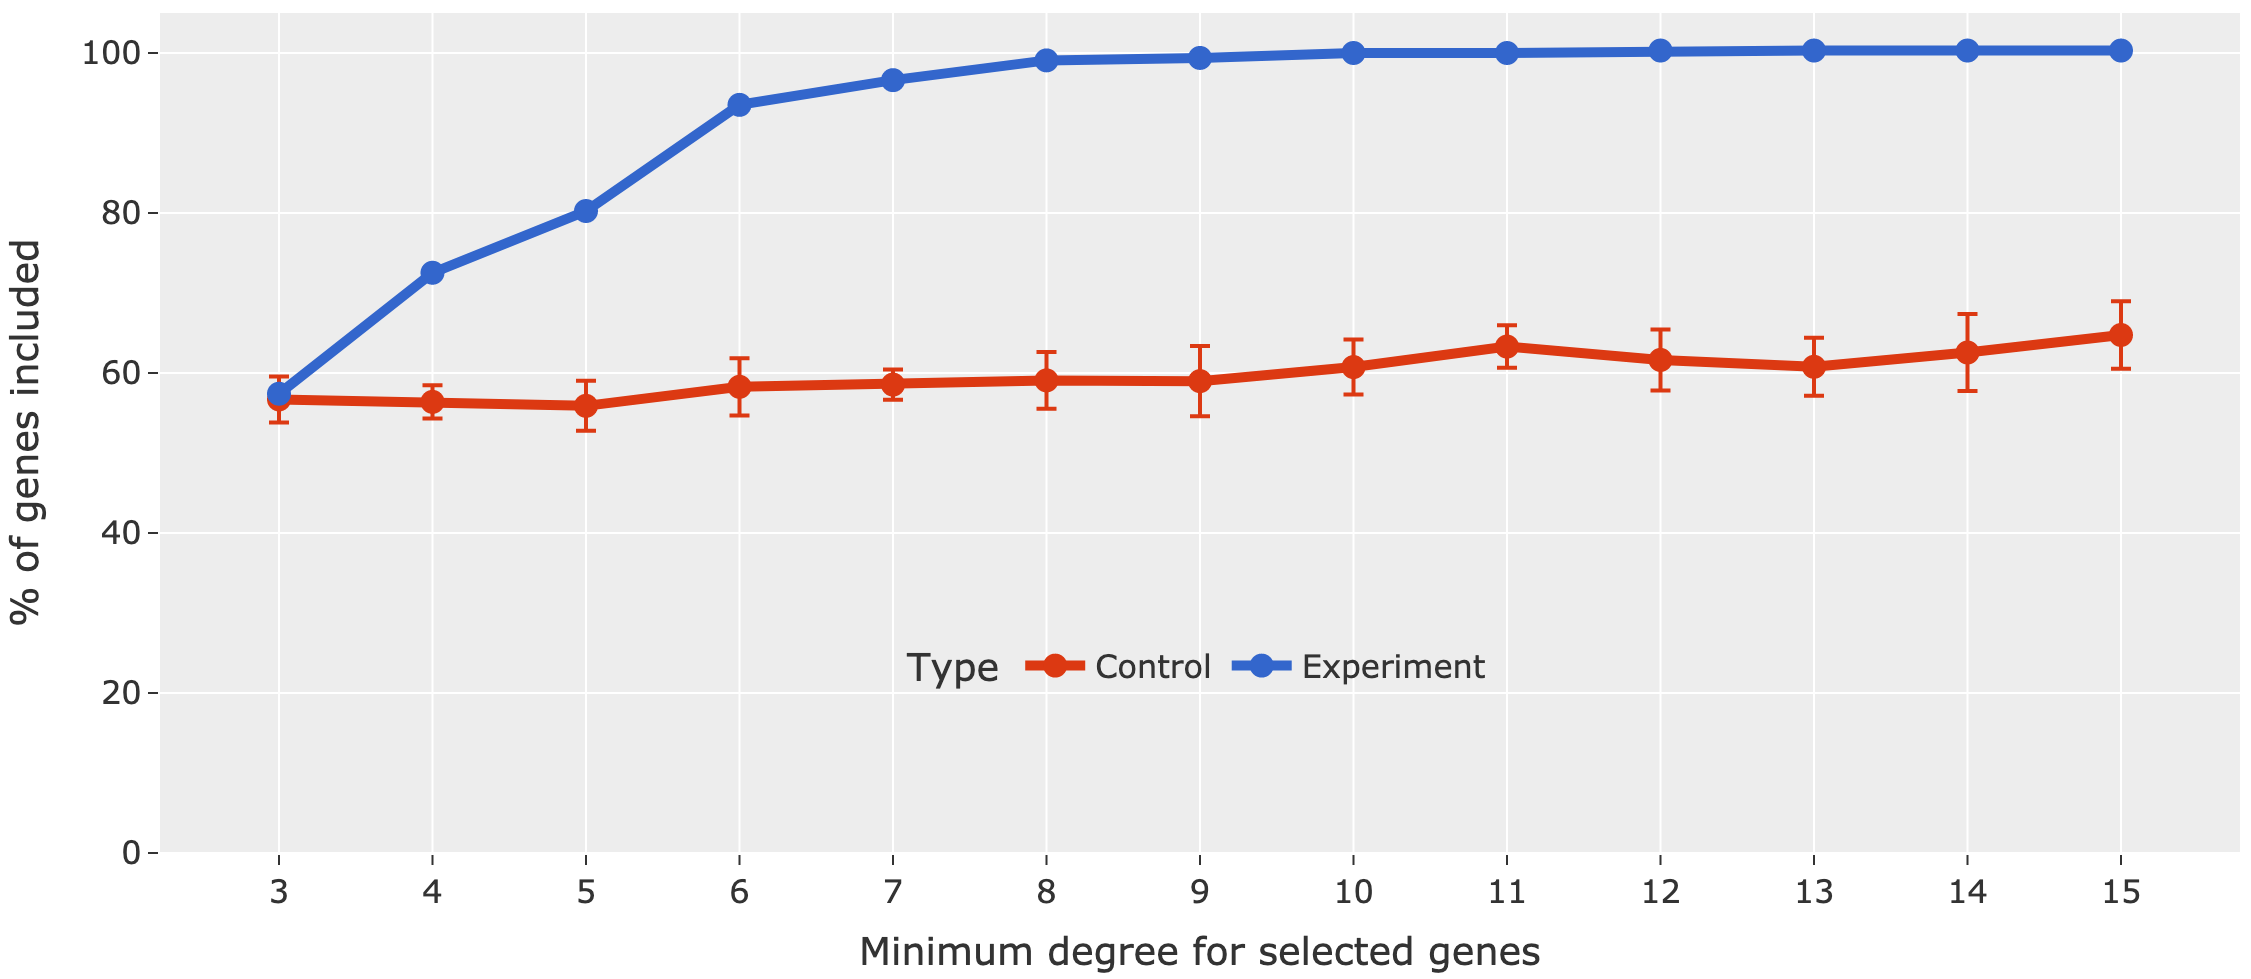
\includegraphics[width=1.0\textwidth,height=1.0\textheight,keepaspectratio]{Sections/Network_I/Resources/selective_pruning/com_comp/ctrls_min_dig_mev.png}
      \caption{The percentages of the Transcription Factors selected by ModCon from the communities found with \acrlong{sbm} as the minimum degree increases. By having $\sim60\%$ of the Transcription Factors selected by ModCon the plot shows there is a subset of TFs that are 'naturally' highly correlated with other genes. }
    \label{fig:N_I:sel_tfs}
\end{figure}

% Biological relevance
% -- Because 50% of the TF naturally emerges and used for subtyping
On contrast to the Experiment trace, the Control appears to have a constant number of biological TFs selected by ModCon, of $\sim60\%$. This means that there is a subset of TFs which are consistently selected by ModCon (i.e. with a high connectivity) despite other than 325 TFs were allowed a high number of connections. 

% Highlighting the importance
To explain this behaviour, it is worth re-surfacing the selective edge pruning process. For each gene in the correlation matrix only the 3 highest correlated genes are kept for standard genes or 6 for the selected genes to prioritise. Thus, a gene can have a starting degree either of 3 or 6. For a node $A$ to have higher a degree, it needs that other genes to have node A in their top correlation. For example, if node $A$ is a non-TF gene and it has a degree value of 10, it means that 7 other genes have node $A$ in their top correlations

% Biological significance
Taking in account the selective edge pruning and that $\sim60\%$ of the 325 TF genes are selected by ModCon, when the TF are \textbf{explicitly} not prioritised, it is remarkable to have a subset of genes that emerged as being highly connected. To further refine the list, the intersection of genes across the controls is taken and this leads to a list of 98 TF, that are constantly highly connected across the controls. The next section analysis this list of TF in depth. 

\begin{figure}[!ht]   
\centering
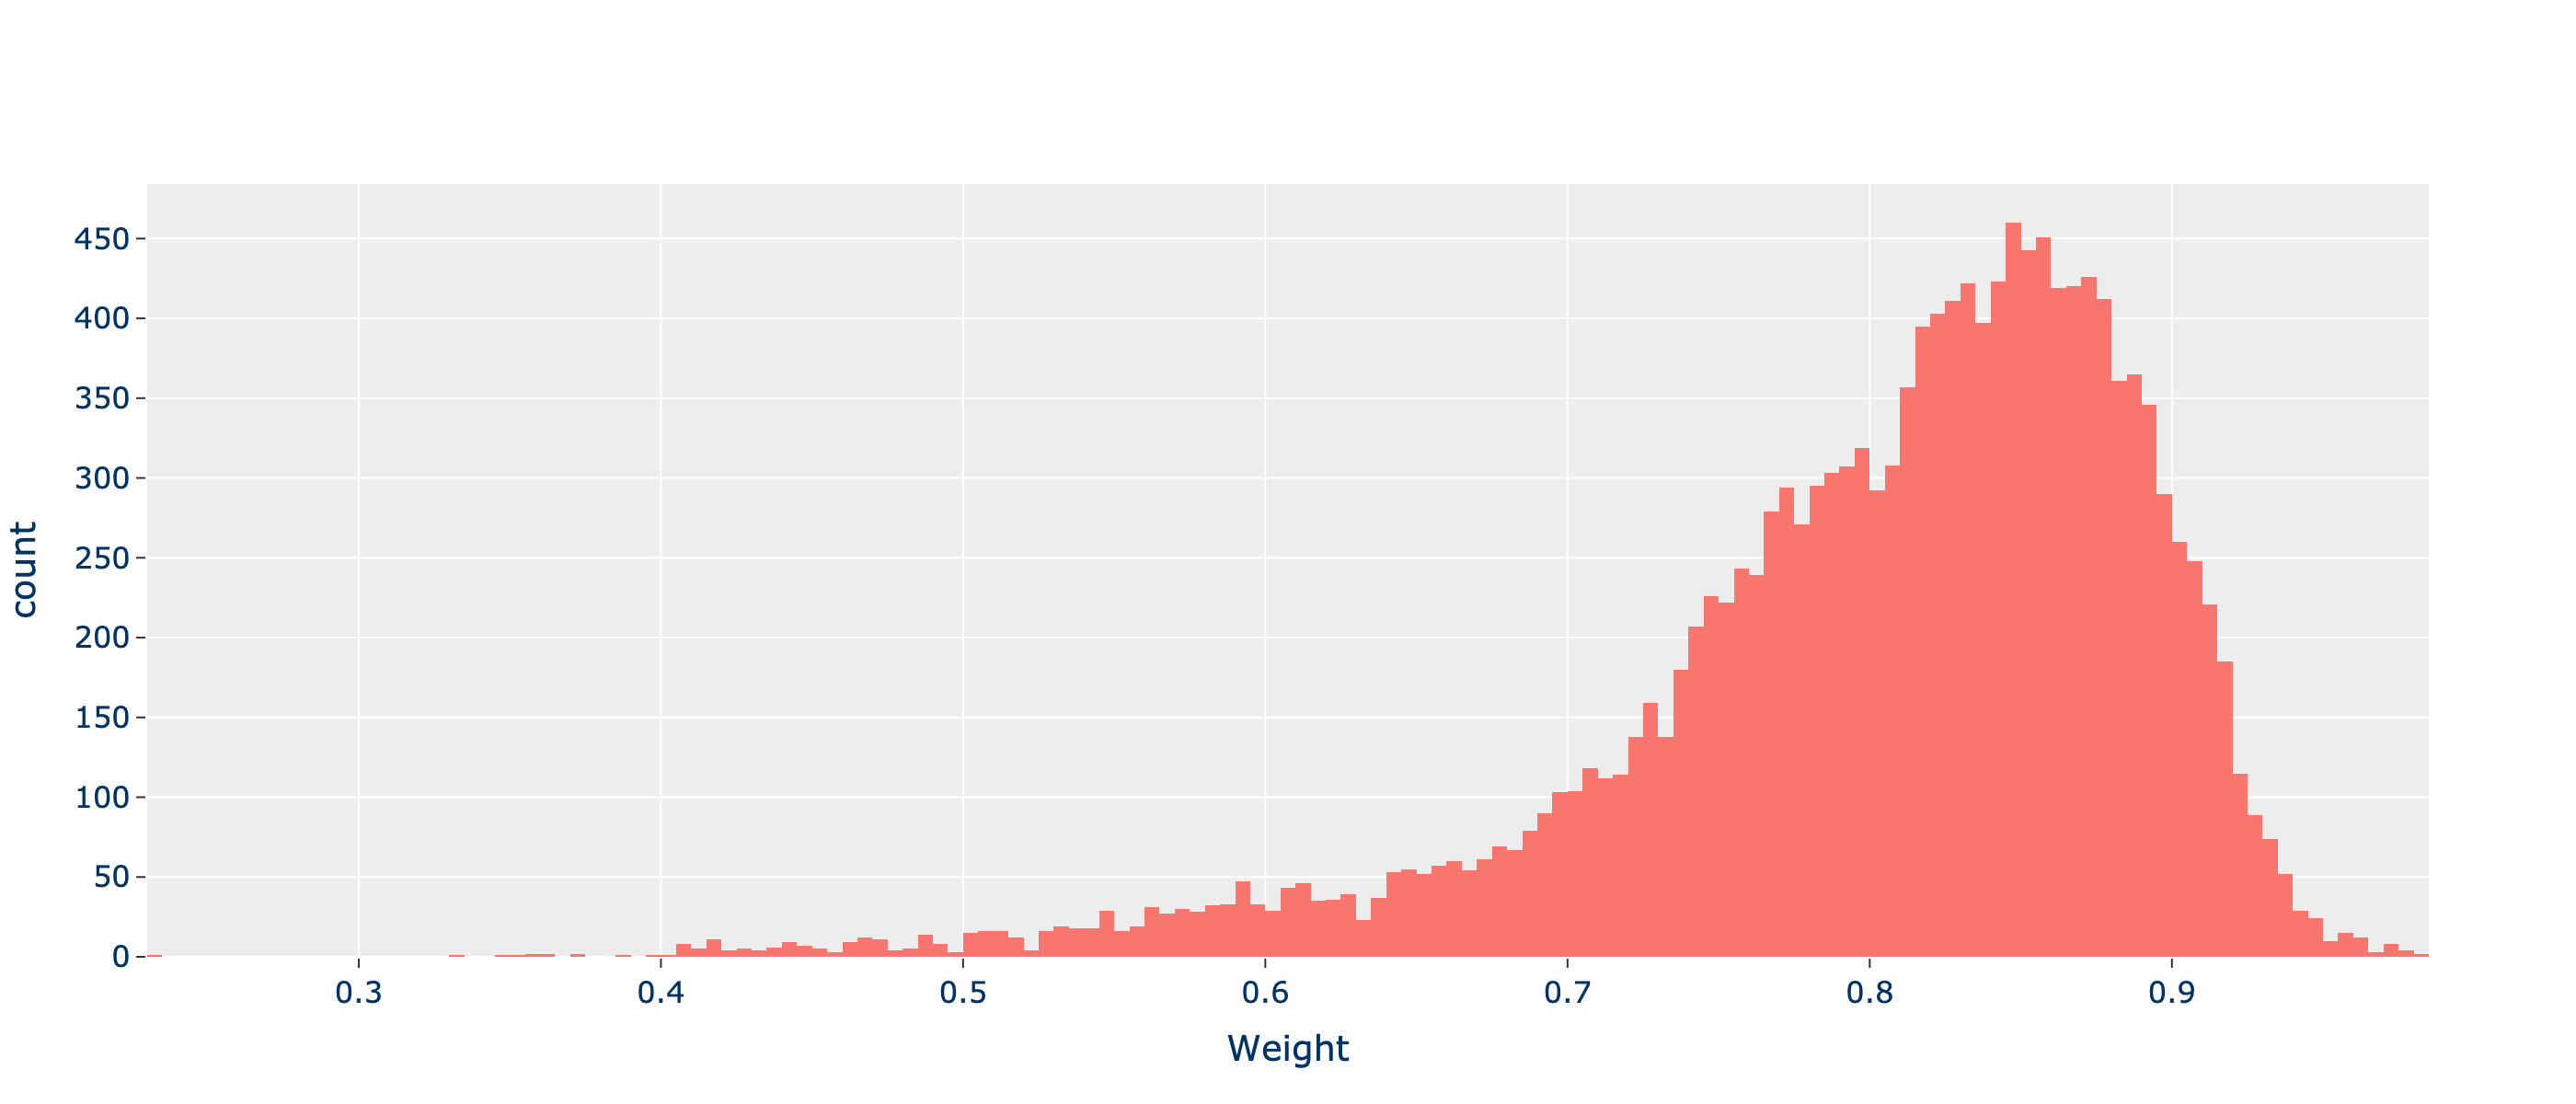
\includegraphics[width=1.0\textwidth,height=1.0\textheight,keepaspectratio]{Sections/Network_I/Resources/selective_pruning/weight_distrib.png}
  \caption{The weight distribution of the edges weights in a standard network (no weight modifier), with 3 edges for non-TF and 6 for TF genes. The distribution is skewed to the left showing that the selective edge prune keeps only the highly correlated pairs of genes.}
\label{fig:N_I:weight_distrib}
\end{figure}

% Shows that the selective edge pruning only selects the highly correlated genes
In the selective edge pruning strategy introduced by \citet{Care2019-ij} there is no threshold to ensure that the low correlated pair of genes are not cluttering the network and that the most co-expressed pairs are kept. To test this the weight distribution is plot in \cref{fig:N_I:weight_distrib} for a standard network with no weight modifiers, with a minimum 3 edges per standard gene and 6 per TF. It can be seen that the distribution is skewed right, ensuring that most of the genes are highly correlated.

% Clustering
\subsection{Clustering analysis}


% Talk about the clustering
Hierarchical clustering was applied to the tumour expression of the 98 TFs after 11 samples previously identified as outliers were removed\footnote{In this context, outliers are samples that cluster in 1-3 groups, making it hard to interpret the dendrogram from the hierarchical clustering}, leaving 392 samples for clustering. The tumour\footnote{TCGA's MIBC cohort} data was log2(TPM+1) transformed, normalised by the quantiles, and then agglomerative clustering with average linkage was applied on the 1-Pearson correlation distance\footnote{In this case, for both clustering and visualisation, Morpheus from the Broad Institute was used \cite{Broad-InstituteUnknown-kn}}. This method was preferred over those developed in the previous chapter because the number of genes was small and the heatmap from Morpheus is a useful tool for showing the gene expression specific to a group. The heatmap and the output are shown in \cref{fig:ap:morph_sel_tfs} in the Appendix.

% describe morpheus
A dendrogram cut of 15 was chosen as it split both the Luminal and Basal Groups and there are relatively small groups. From the heatmap \cref{fig:ap:morph_sel_tfs} it can be noticed that there is a large group of Luminal samples and a smaller one. The Basal group is split into three subgroups, a large one, a medium size which groups most of the Mes-like tumours from Lund classifier and a smaller ones which has a lower Infiltration/Stromal/Estimate scores compared to the other 2 Basal groups. Apart from these 2 groups, there are outliers samples that are grouped in 1 or 2 clusters, suggesting that they have particular molecular profiles.

\begin{figure}[!t]
\centering
    \centering
    % Sankey - consensus and K-means comparison
    \begin{subfigure}[!t]{1.0\textwidth}
        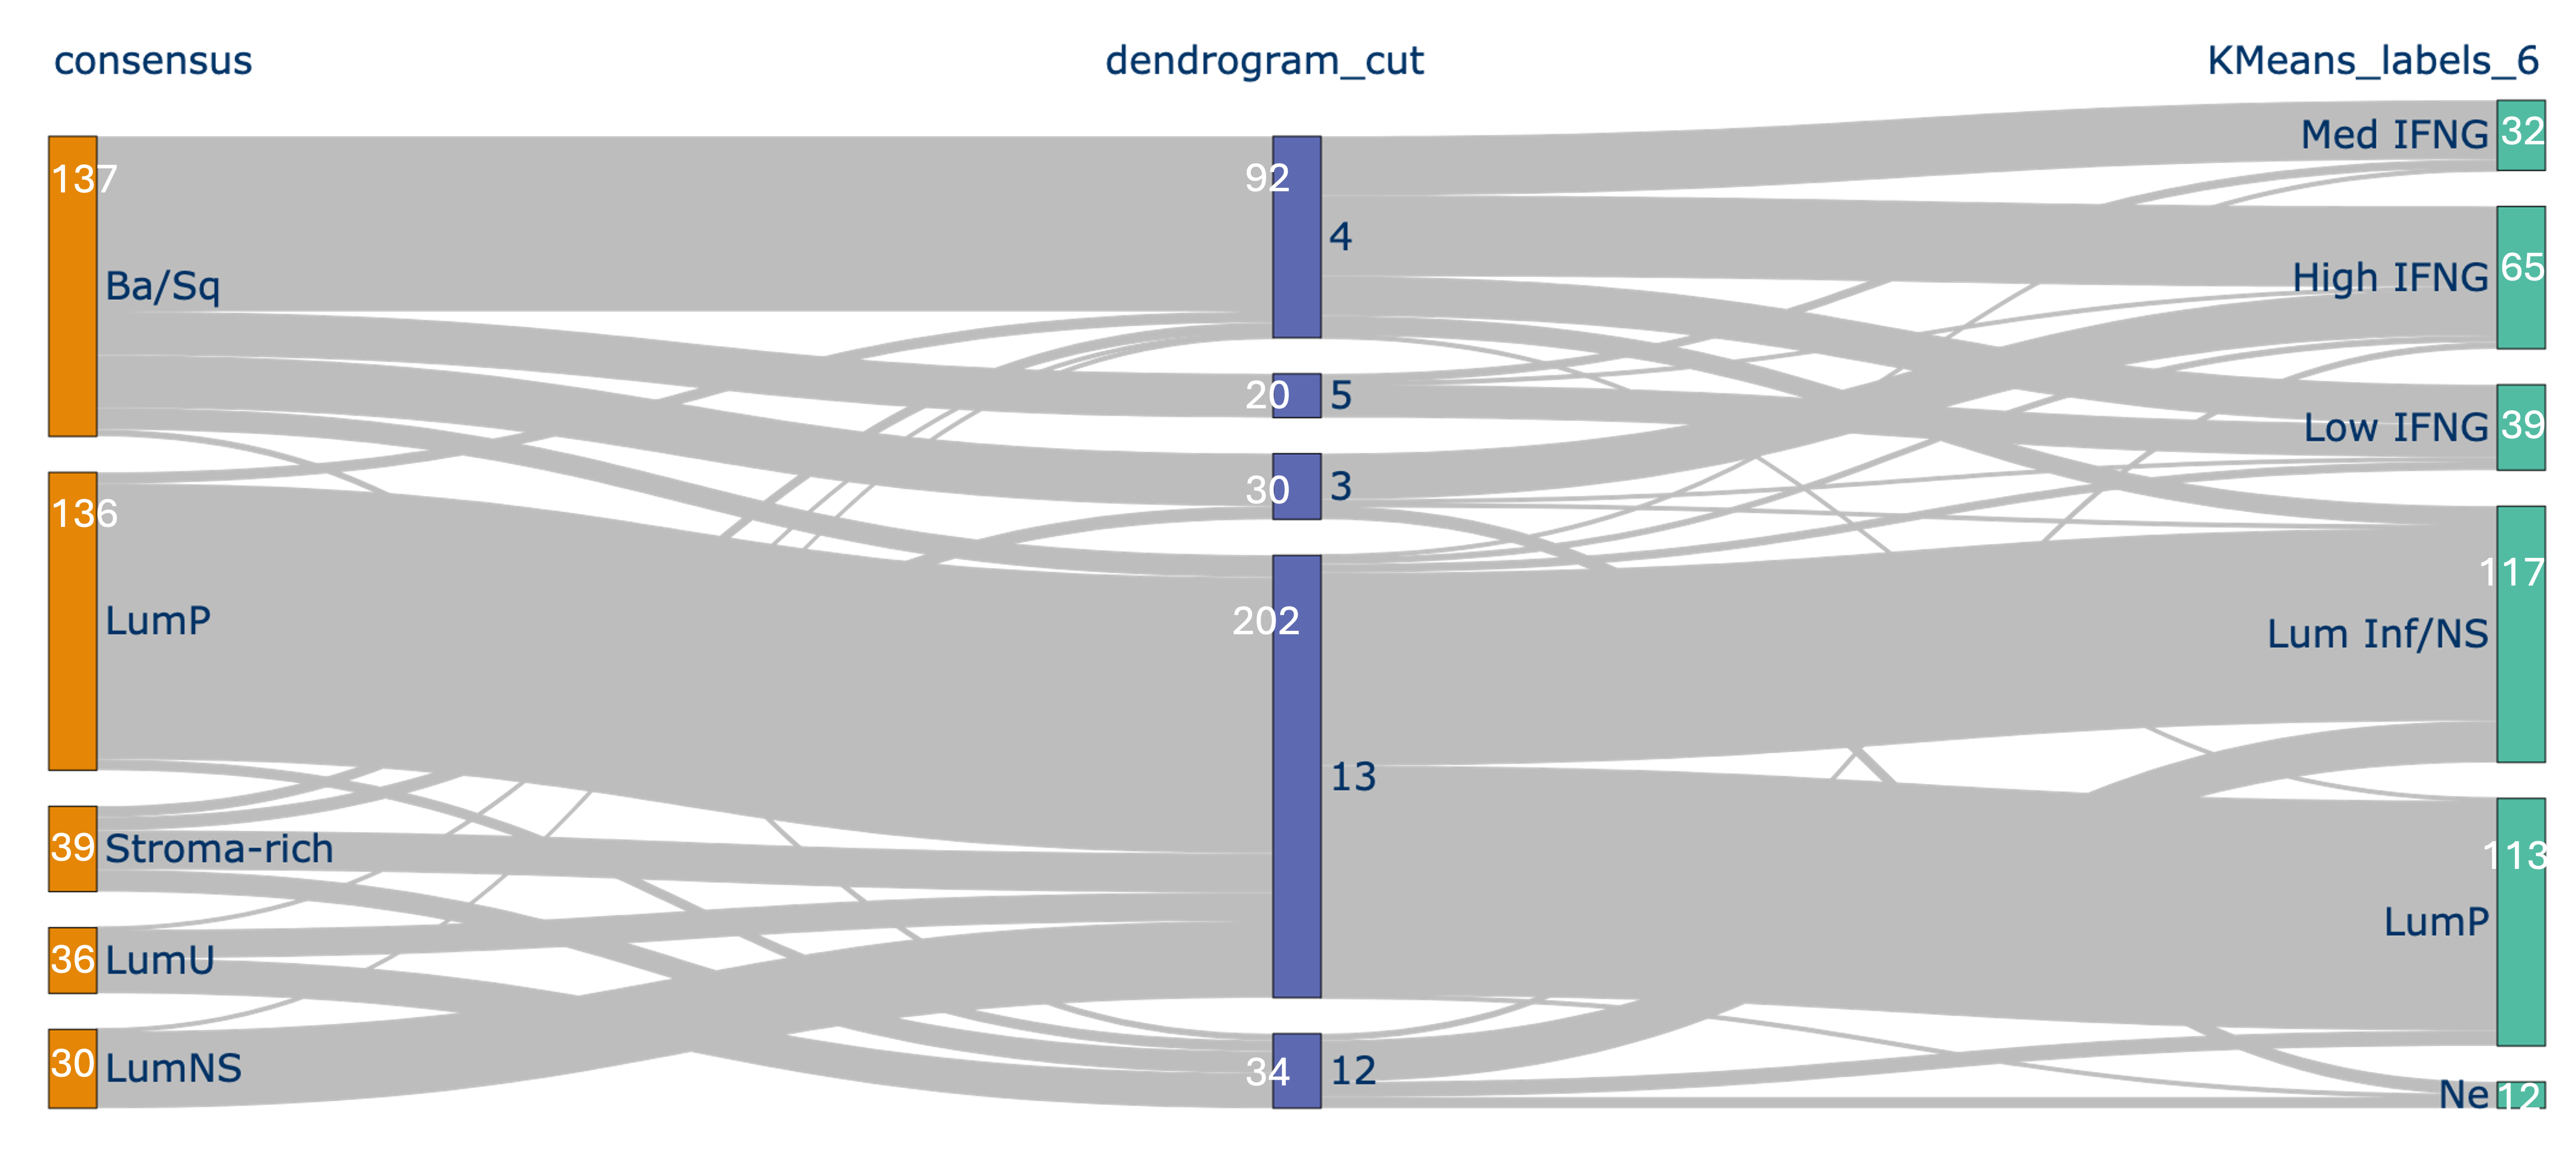
\includegraphics[width=1.0\textwidth,keepaspectratio]{Sections/Network_I/Resources/selective_pruning/sel_tfs/sankey_sel_tfs_VU_CS.png}
        \caption{Sankey plot comparison between the hierarchical clustering from \cref{fig:ap:morph_sel_tfs}, consensus \cite{Kamoun2020-tj} and clustering performed in the earlier chapter \cref{s:lit:clustering}.}
        \label{fig:N_I:sankey_sel_tfs_vuCs}
    \end{subfigure}
    % Sankey - TCGA and Lun comparison  
    \begin{subfigure}[!t]{1.0\textwidth}
        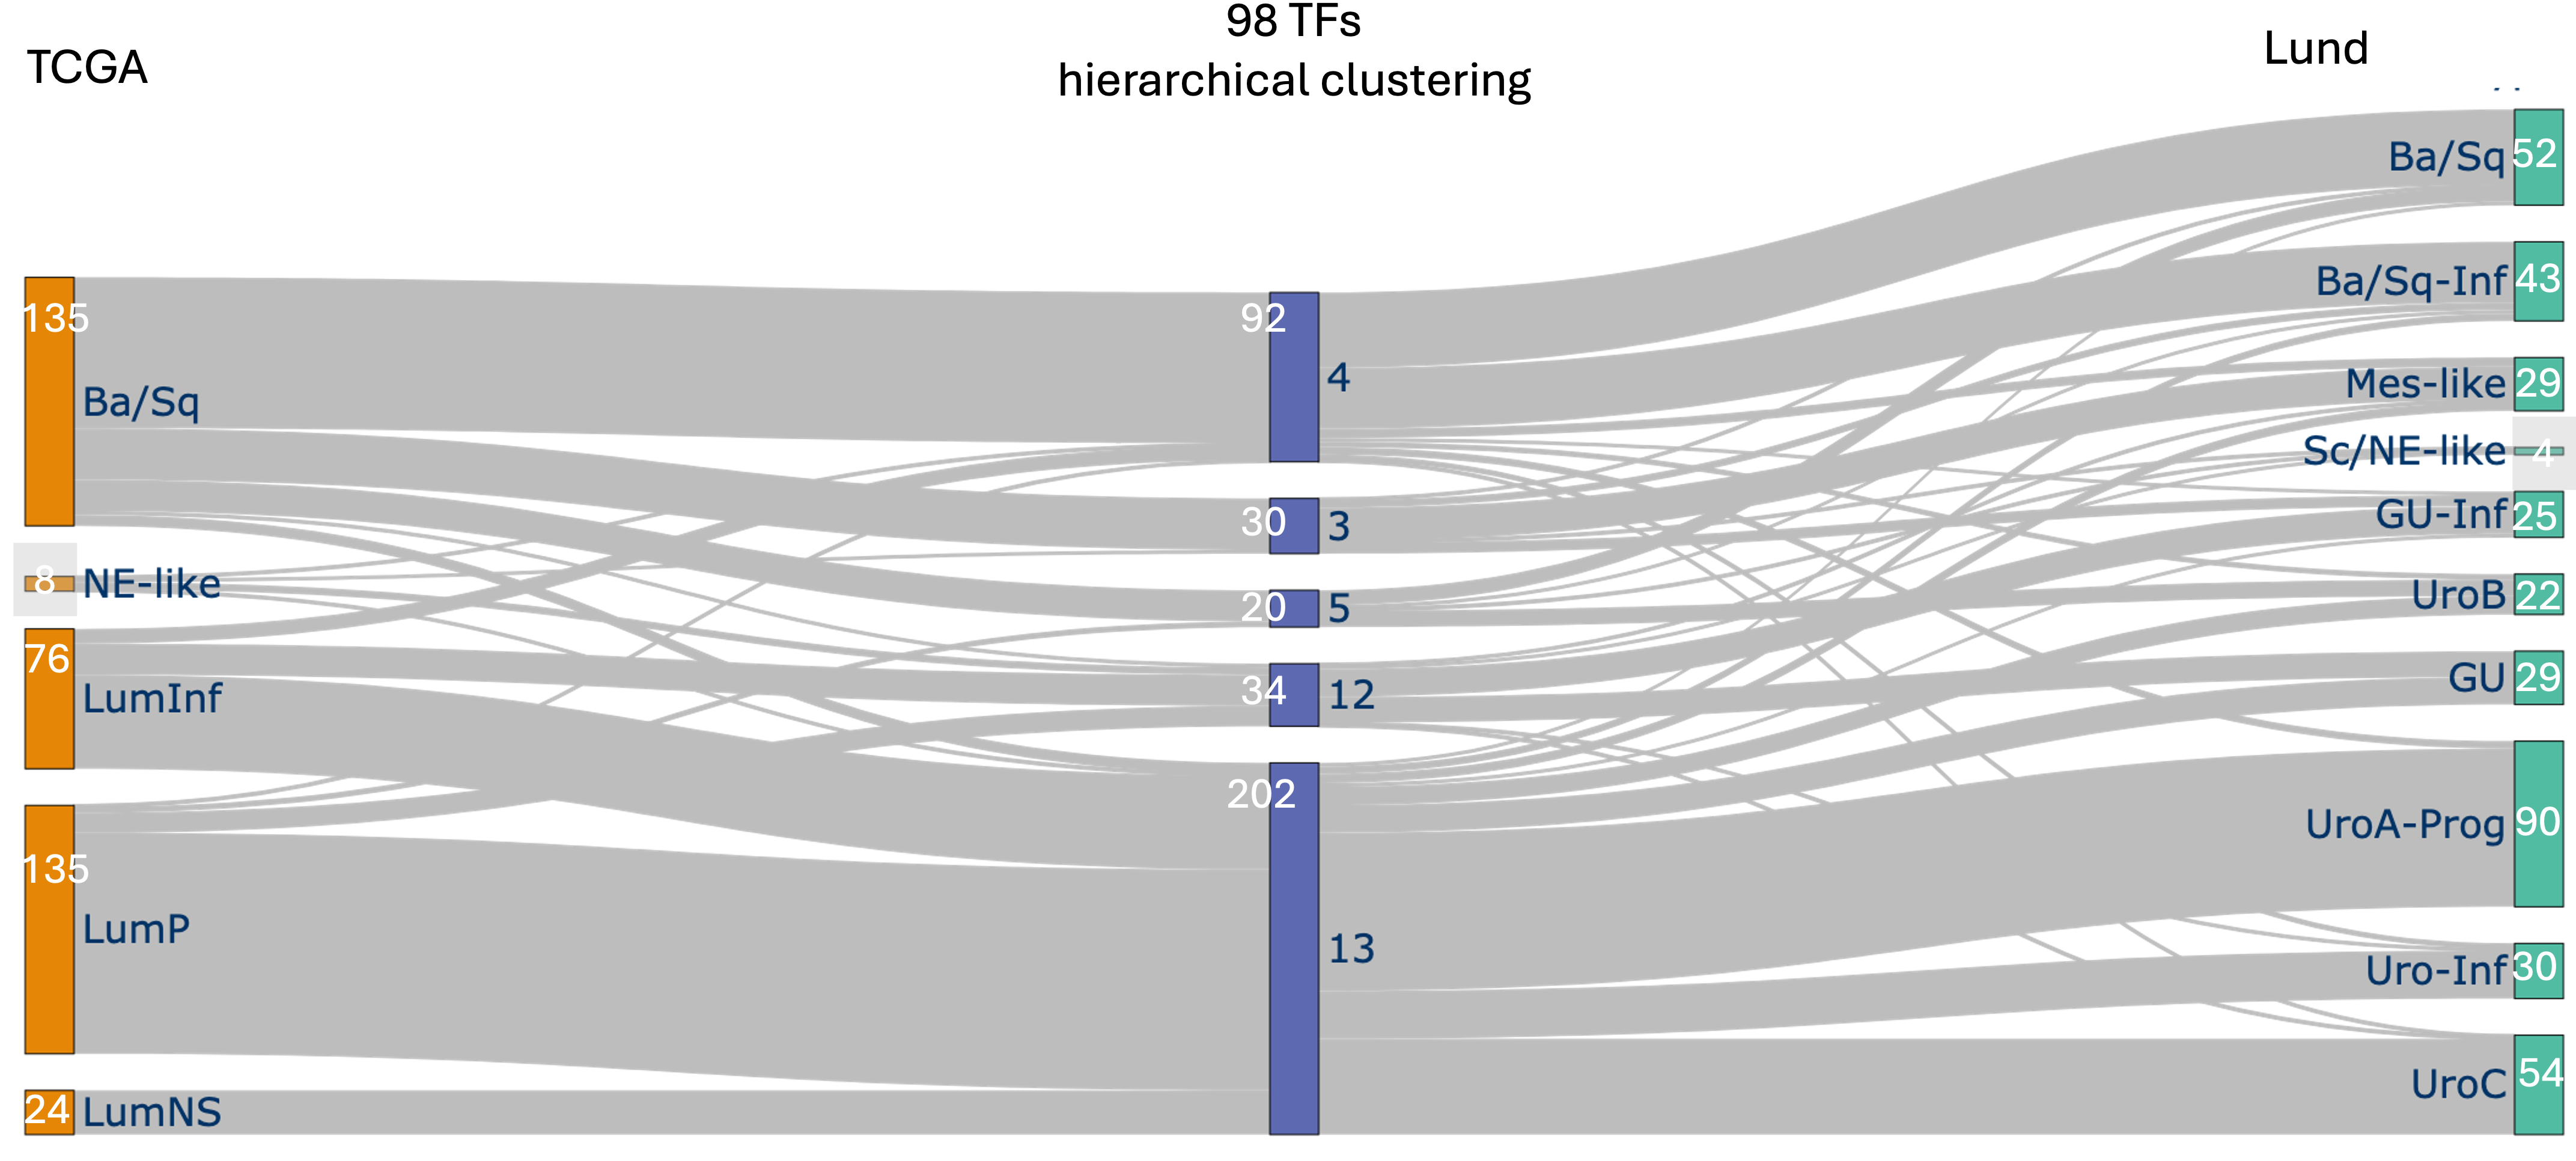
\includegraphics[width=1.0\textwidth,keepaspectratio]{Sections/Network_I/Resources/selective_pruning/sel_tfs/sankey_sel_tfs.png}
        \caption{Sankey plot comparison between the hierarchical clustering from \cref{fig:ap:morph_sel_tfs}, TCGA \cite{Robertson2017-mg} and Lund \cite{Marzouka2018-ge}.}
        \label{fig:N_I:sankey_sel_tfs}
    \end{subfigure}
    % Survival
    \centering
    \caption{Cluster analysis of the subgroups derived using the found 98 TFs. The white text on the Sankey plots represents the size of the groups.}
    \label{fig:N_I:sel_tfs_cs_analysis}
\end{figure}

 
% Describe Sankey
The groups smaller than 1\% of the cohort size (equivalent to 4 samples) are removed, resulting in a dataset of 378 samples grouped into 5 major groups. These subtypes are compared in \cref{fig:N_I:sankey_sel_tfs_vuCs,fig:N_I:sankey_sel_tfs} with previous work from Lund \citep{Marzouka2018-ge}, TCGA \citep{Robertson2017-mg}, consensus \citep{Kamoun2020-tj}, and the subtyping clusters found in the previous chapter on clustering analysis \cref{s:clustering_analysis}. 

% Luminal groups
In the comparison (\cref{fig:N_I:sankey_sel_tfs_vuCs}) with the consensus and the clusters from the previous section \cref{s:clustering_analysis}, it can be noticed that there is a large luminal group (13) consisting of 202 samples. The group contains most, if not all, of the samples from LumP, Stroma-rich, LumU, and LumNS (consensus) and the LumInf/NS and LumP (KMeans\_6). This is also the case in \cref{fig:N_I:sankey_sel_tfs}, where group 13 contains the LumInf, LumP, LumNS (TCGA) and the UroA-Prog, Uro-Inf, and UroC from Lund. The smaller luminal group (12) consists mostly of the samples from LumU, Stroma-rich from TCGA (\cref{fig:N_I:sankey_sel_tfs_vuCs}) or the consensus LumInf/LumP (TCGA) or the Genomically Unstable (GU) and GU-infiltrated from Lund. 

% Basal subgroups
The larger group, consisting of 92 samples, is formed of a mix of samples from Medium, High, and Low IFNG (KMeans\_6) and Ba/Sq samples from the consensus. The medium-sized group is a combination of the High IFNG and Ne subgroups from KMeans\_6, while the smaller-sized group is formed of Low IFNG and Med IFNG. Switching to the comparison with TCGA/Lund (\cref{fig:N_I:sankey_sel_tfs}), it can be noticed that the large basal group (4) contains most of the Ba/Sq (TCGA) or Ba/Sq and Ba/Sq-infiltrated (Lund) samples. The medium-sized (3) basal cluster contains most of the Mes-like samples (Lund), while the smaller group (5) consists of UroB and Ba/Sq (Lund) samples. Thus, the MIBC stratification on the 98 TFs exhibits one major (large) basal group (4), a medium-sized (3) group which contains the Mes-like samples from the Lund classifier or the samples from High IFNG, and the small basal group (5) consisting of low IFNG samples or a combination of the UroB and Ba/Sq samples. It is worth mentioning that the UroB (Lund) and Low IFNG have a low survival prognosis, while High IFNG has a good prognosis.

% Summary of the comparison
The comparison with the other stratification methods shows that clustering the expression of 98 TFs is capable of finding three basal subtypes, two smaller even than the ones found in the previous cluster analysis from \ref{s:clustering_analysis}. However, the 98 TFs fail to discriminate the luminal subgroups.

% Survival analysis
\subsection{Survival Analysis}

Survival analysis was conducted on the five groups derived from the 98 transcription factors as shown in \cref{fig:N_I:sel_tfs_survival}. Group 5, identified as the smallest basal group, exhibits the poorest survival prognosis by a significant margin. Notably, the poorest survival in both the TCGA and consensus classification is observed in the Neuroendocrine-like groups, which are not included in Group 5; this is illustrated in the Sankey plot in \cref{fig:N_I:sankey_sel_tfs}. It is striking the poor survival of the group 5, where almost all of the patients are deceased after 3 years. This is a poorer prognosis then the Lund's UroB subtype (see Figure 6 from \citet{Marzouka2018-ge}) and the Low IFNG Basal from \ref{}.

The largest luminal group (13) demonstrates the best overall prognosis, followed by the medium-sized basal cluster or Mes-like (3). The luminal infiltrated group (12) shows survival trends similar to clusters 3, 4, and 12, but the survival prognosis deteriorates over a five-year period. The multivariate log-rank test, yielding a $p<0.005$, confirms the statistical significance of the differences in survival among the five groups.

% Giving context to the results
The clustering analysis shows that the by only using 98 genes, the main groups, Basal and Luminal, are discovered. The survival analysis indicates that these subtypes have significantly different survival prognosis. The gene expression heatmap from \cref{fig:ap:morph_sel_tfs} reveals that there some highly varied genes\footnote{This is given by the rows that are either completely blue or red (\textit{BNC1, FOXJ3, ELF3}), suggesting that there }, which was also previously observed in \cref{fig:N_I:sel_tfs_var}. 


\begin{figure}[!t]
    \centering
    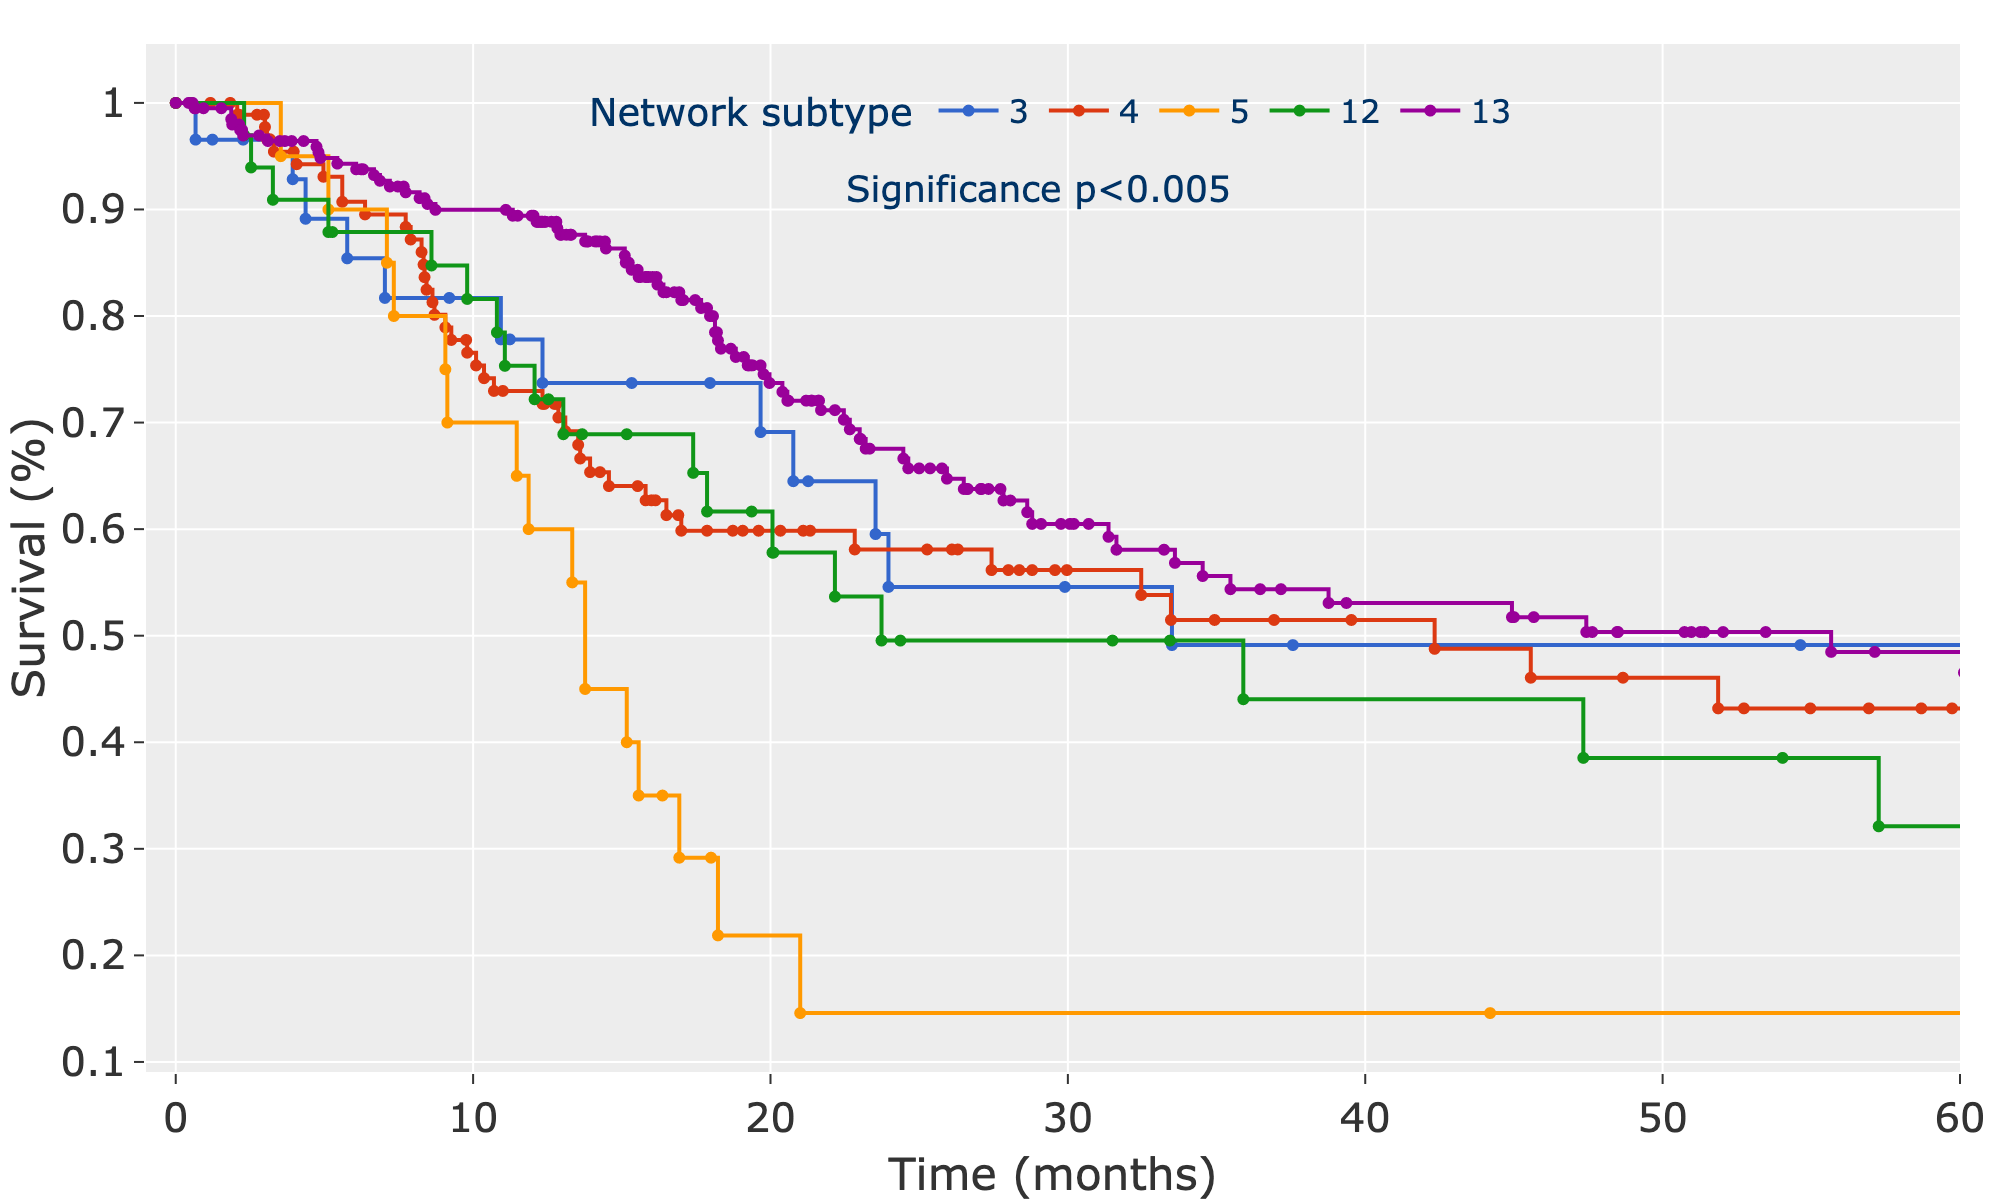
\includegraphics[width=1.0\textwidth,keepaspectratio]{Sections/Network_I/Resources/selective_pruning/sel_tfs/survival_sel_tfs_cs.png}
    \caption{Kaplan-Meier survival analysis of the MIBC subtypes derived from the expression of the 98 TFs. The multivariate long rank test found a significant difference of 0.000140 between the survival of the five groups. Group 5 have one of the lowest survival prognosis seen in the literature. }
    \label{fig:N_I:sel_tfs_survival}
\end{figure} 


% the biggest change
The dumbbell figure in \cref{fig:N_I:dumbell_sel_tfs} exhibit the difference in expression between subgroups. Each point represents the $log2(mean\_TPM+1)$ and the subplots are in descending order of the fold change between the two averages. The largest changes happen between the basal-like (4,5) and luminal-like (13, 12) subgroups as well as between mes-like (3) \& basal-like groupsl; see A) and C). The least changes happen in B) where the main group of Luminal is compared with the 'infiltrated' version, exhibiting a change in magnitude of expression rather then a major difference.  \Cref{fig:N_I:dumbell_sel_tfs} A) and C) shows that \textit{BNC1} is absent in both Luminal groups. This gene also is low expressed in the basal subtypes comparison with the mes-like gorup in D) and E). \textit{BNC1} is a squamous cell marker as shown by the work of \citet{Hurst2022-sp}.

\textit{TP63} is a known Squamous marker \citet{Robertson2023-na} and indirectly of un-differentiation status. The difference in expression between subgroups is the most evident in the comparison of the basal subtypes (C and E) as well as in the small basal vs mes-like (C). The basal groups having higher mean expression than the others, with the highest in the small basal group (F). It is worth noting, that there is little fold change in the basal and luminal comparison (A). The basal groups over the mes-like are characterised by having a higher expression in: \textit{HES2, GRHL3, IRF6, ZNF750, BNC1, OVOL1, KLF5}. The smaller basal group seems to have stronger expression of the basal markers compared to the larger ones.

Overall, there are a few genes that have large changes in the comparison shown in \cref{fig:N_I:dumbell_sel_tfs}: 
\begin{itemize}
    \item \textit{BNC1, MYCL, FOXQ1, HES2, GRHL3 and HOXB6} in the main Basal (4), Luminal (13) comparison
    \item \textit{TP63} between Luminal (13) and Luminal infiltrated (12)
    \item \textit{TP63, BNC1, HES2, MSX2, MYCL, HOXB6, IRF6, GRHL3} - small Basal (5) and Luminal infiltrated (12), \textit{BNC1} being completely unexpressed in the subgroup 12
    \item \textit{TP63, HES2, GRHL3, IRF6, BNC1, ZNF750, ZBTB7C, MYCL} - mes-like (3) vs Basal (4), \textit{BNC1} being unexpressed in the mes-like group
    \item \textit{GRHL3, TP64, HES2, IRF6, ZBTB7C, ZNF750, BNC1, OVOL1} - mes-like (3) vs small Basal (5) 
    \item \textit{ZBTB7C, MECOM, MSX2, TP63, KLF5, ELF3} - large Basal (4) vs small Basal (5); this comparison shows that the smaller basal has higher enriched of basal markers.
\end{itemize}


It is know that \textit{MYCL, GRHL3, HOXB6, KLF5, ELF3} are involved in bladder differentiation, \textit{TP63} is a marker for undifferentiated and squamous tumours in MIBC as well as \textit{HES2}. The surprising TF is \textit{BNC1} which is completely un-expressed in the luminal tumours and expressed in the Basal subgroups; admittedly not very high as shown in \cref{fig:ap:sel_tfs_mean}. This suggests that many of the mentioned TFs may have a role in tissues differentiation.

This preliminary analysis of the differences in gene expression between subtypes indicates the presence of significant biological insights to be uncovered from the subgroups derived using the 98 TFs. This is further supported by the notable survival disparity observed in the small basal group, as shown in \cref{fig:N_I:sel_tfs_survival}. The subsequent section aims to refine the list of 98 TFs and to investigate the underlying biology of each MIBC subtype.

% \begin{figure}[!ht]   
\begin{sidewaysfigure}

    \centering
    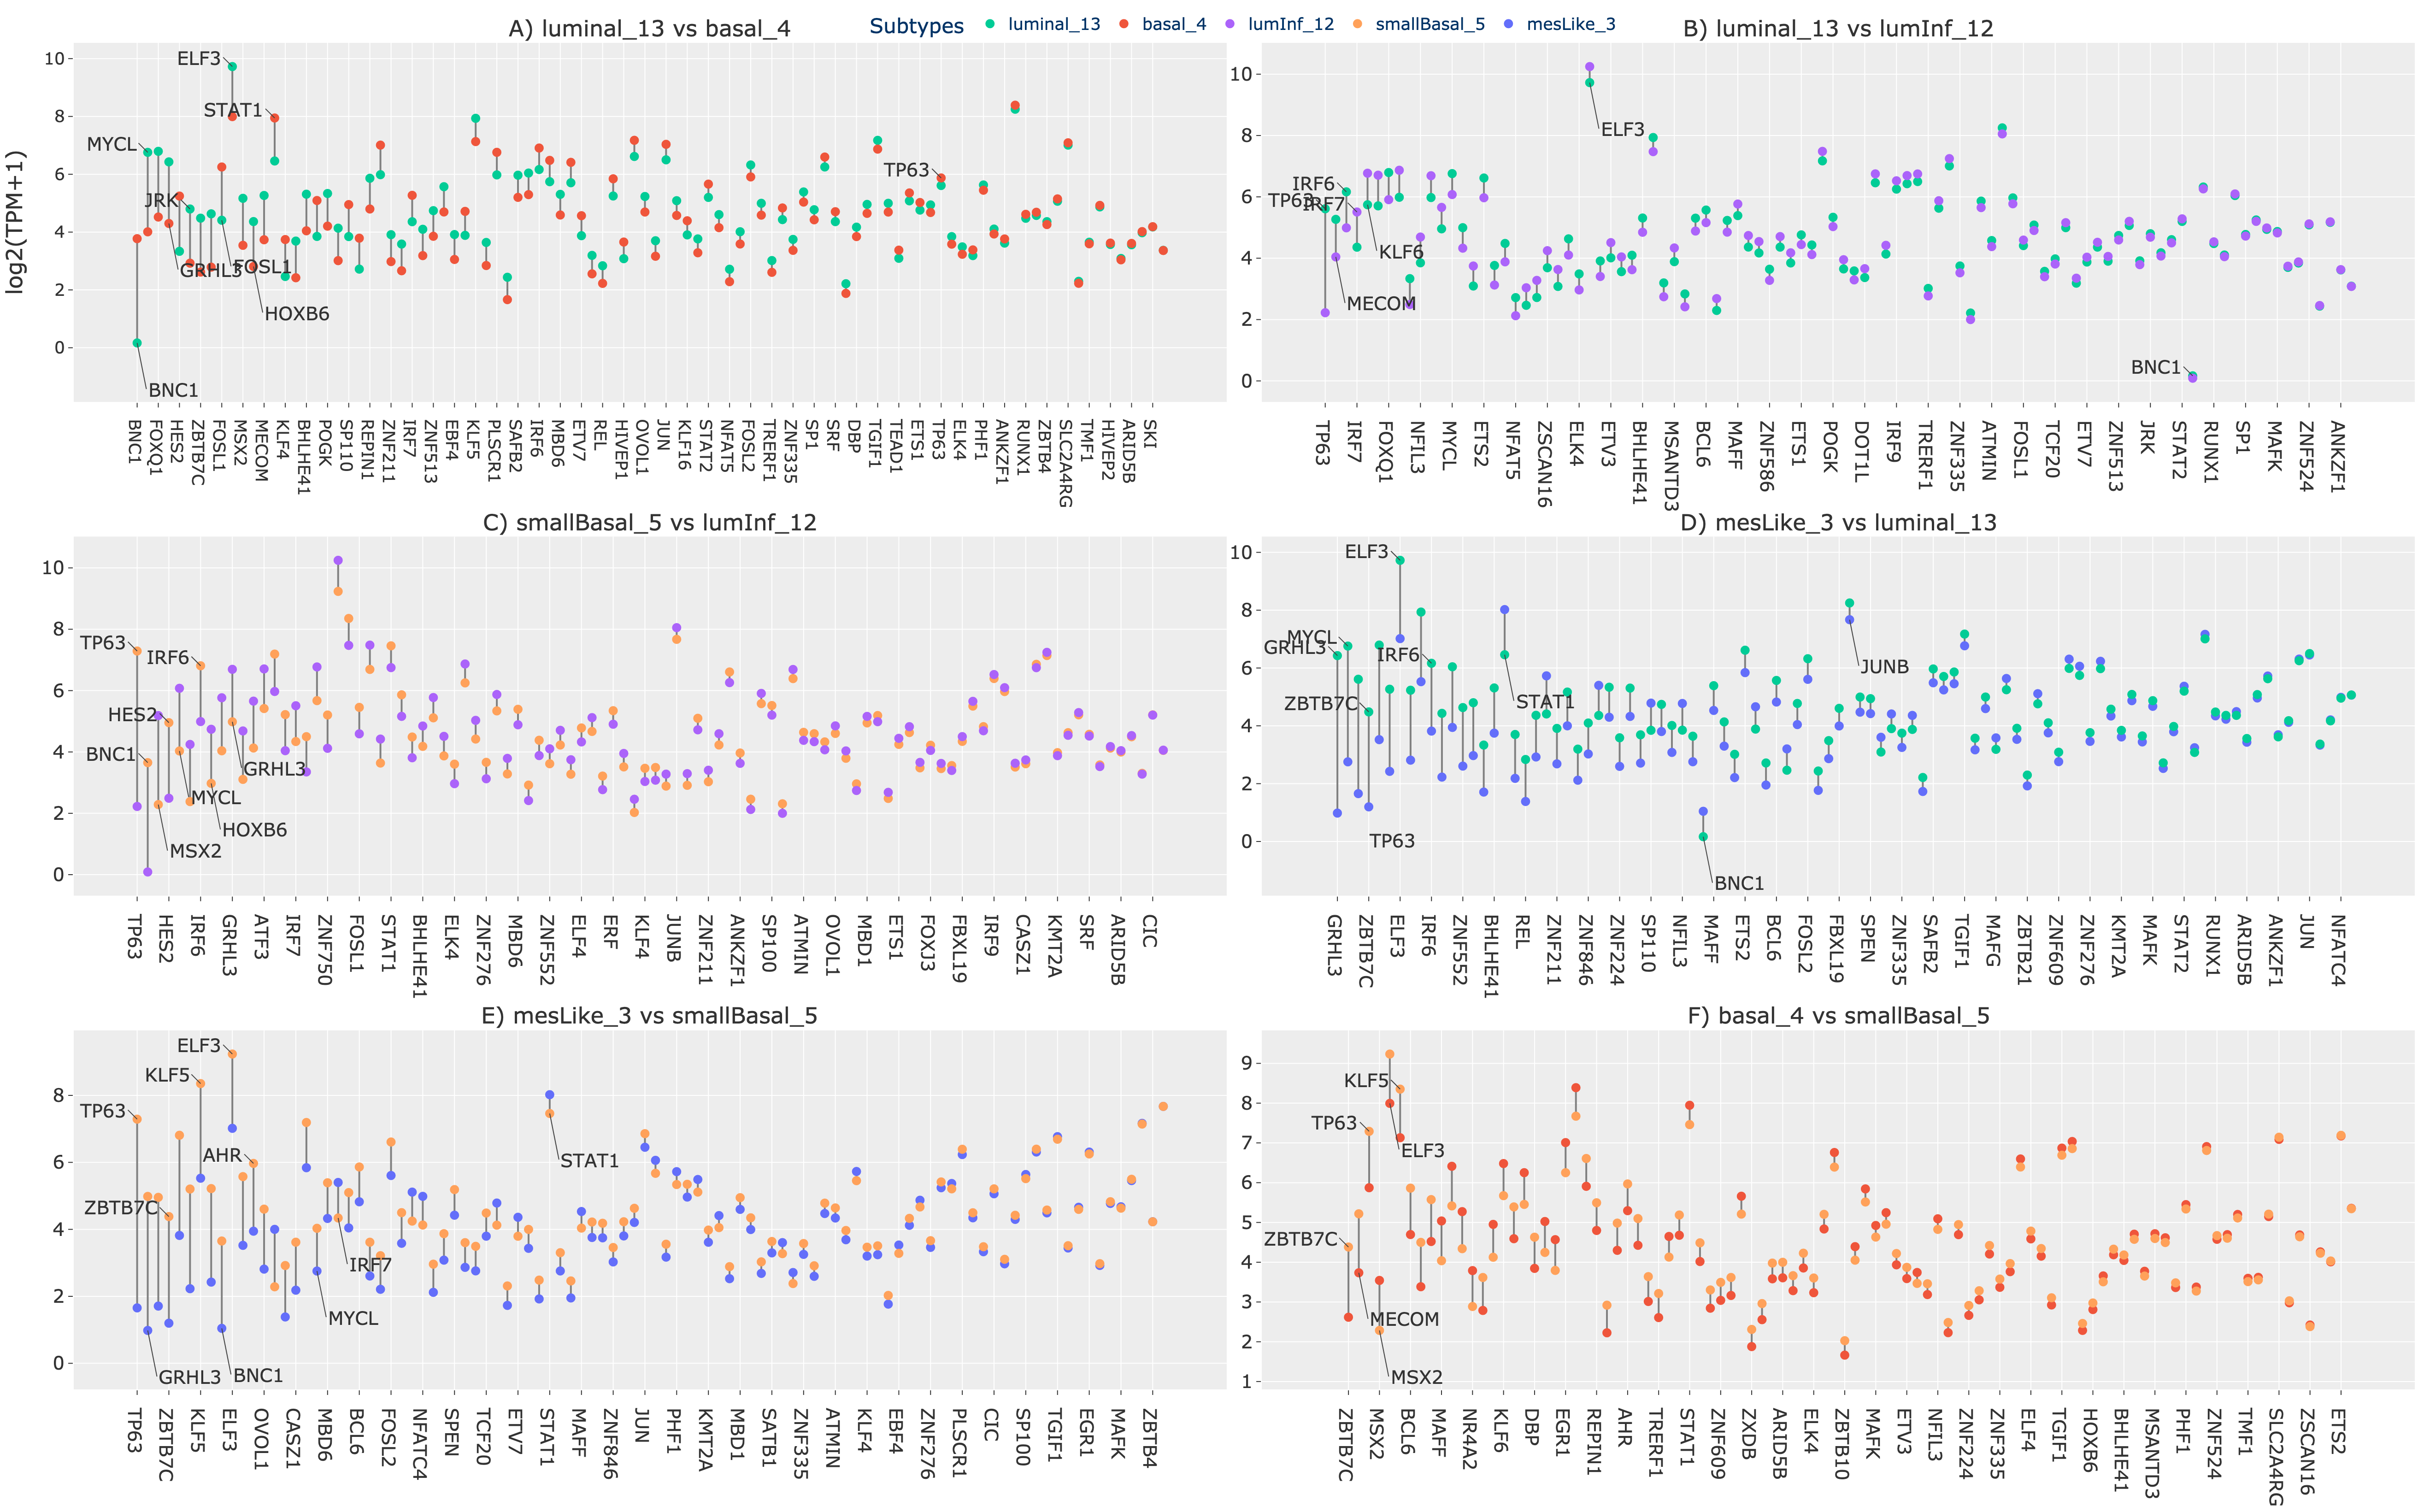
\includegraphics[width=1.0\textwidth,keepaspectratio]{Sections/Network_I/Resources/selective_pruning/dumbell_sel_tfs.png}
      \caption{Comparison of the mean across the subtypes derived with the 98 TFs. Each point represents the $log2(mean\_TPM+1)$ and the subplots are in descending order of the fold change.}
    \label{fig:N_I:dumbell_sel_tfs}
\end{sidewaysfigure}

\newpage




% Biological analysis
\section{Result: the biology behind the emergent TFs} \label{s:N_I:sel_tfs_bio}

The bar plots in \cref{fig:N_I:sel_tfs_var} display the log mean of the gene expression in both non-cancerous and cancerous datasets of the 98 TFs genes. The error bars depict the standard deviation of expression and the genes are in the descending order of the tumour average expressions. The red-bars represent the genes have a high variance\footnote{In this case, a high varied genes is one which has a standard deviation as big as the mean expression} in the either the non-cancerous or tumour dataset and the golden are the genes varied in both. Highly varied genes are the ones highlighted in the bar plot may yield important gene expression markers between the subgroups. The three list of varied genes can be seen \cref{tab:N_I:sel_tfs_var}.

% Variance
\begin{figure}[!htb]   
\centering
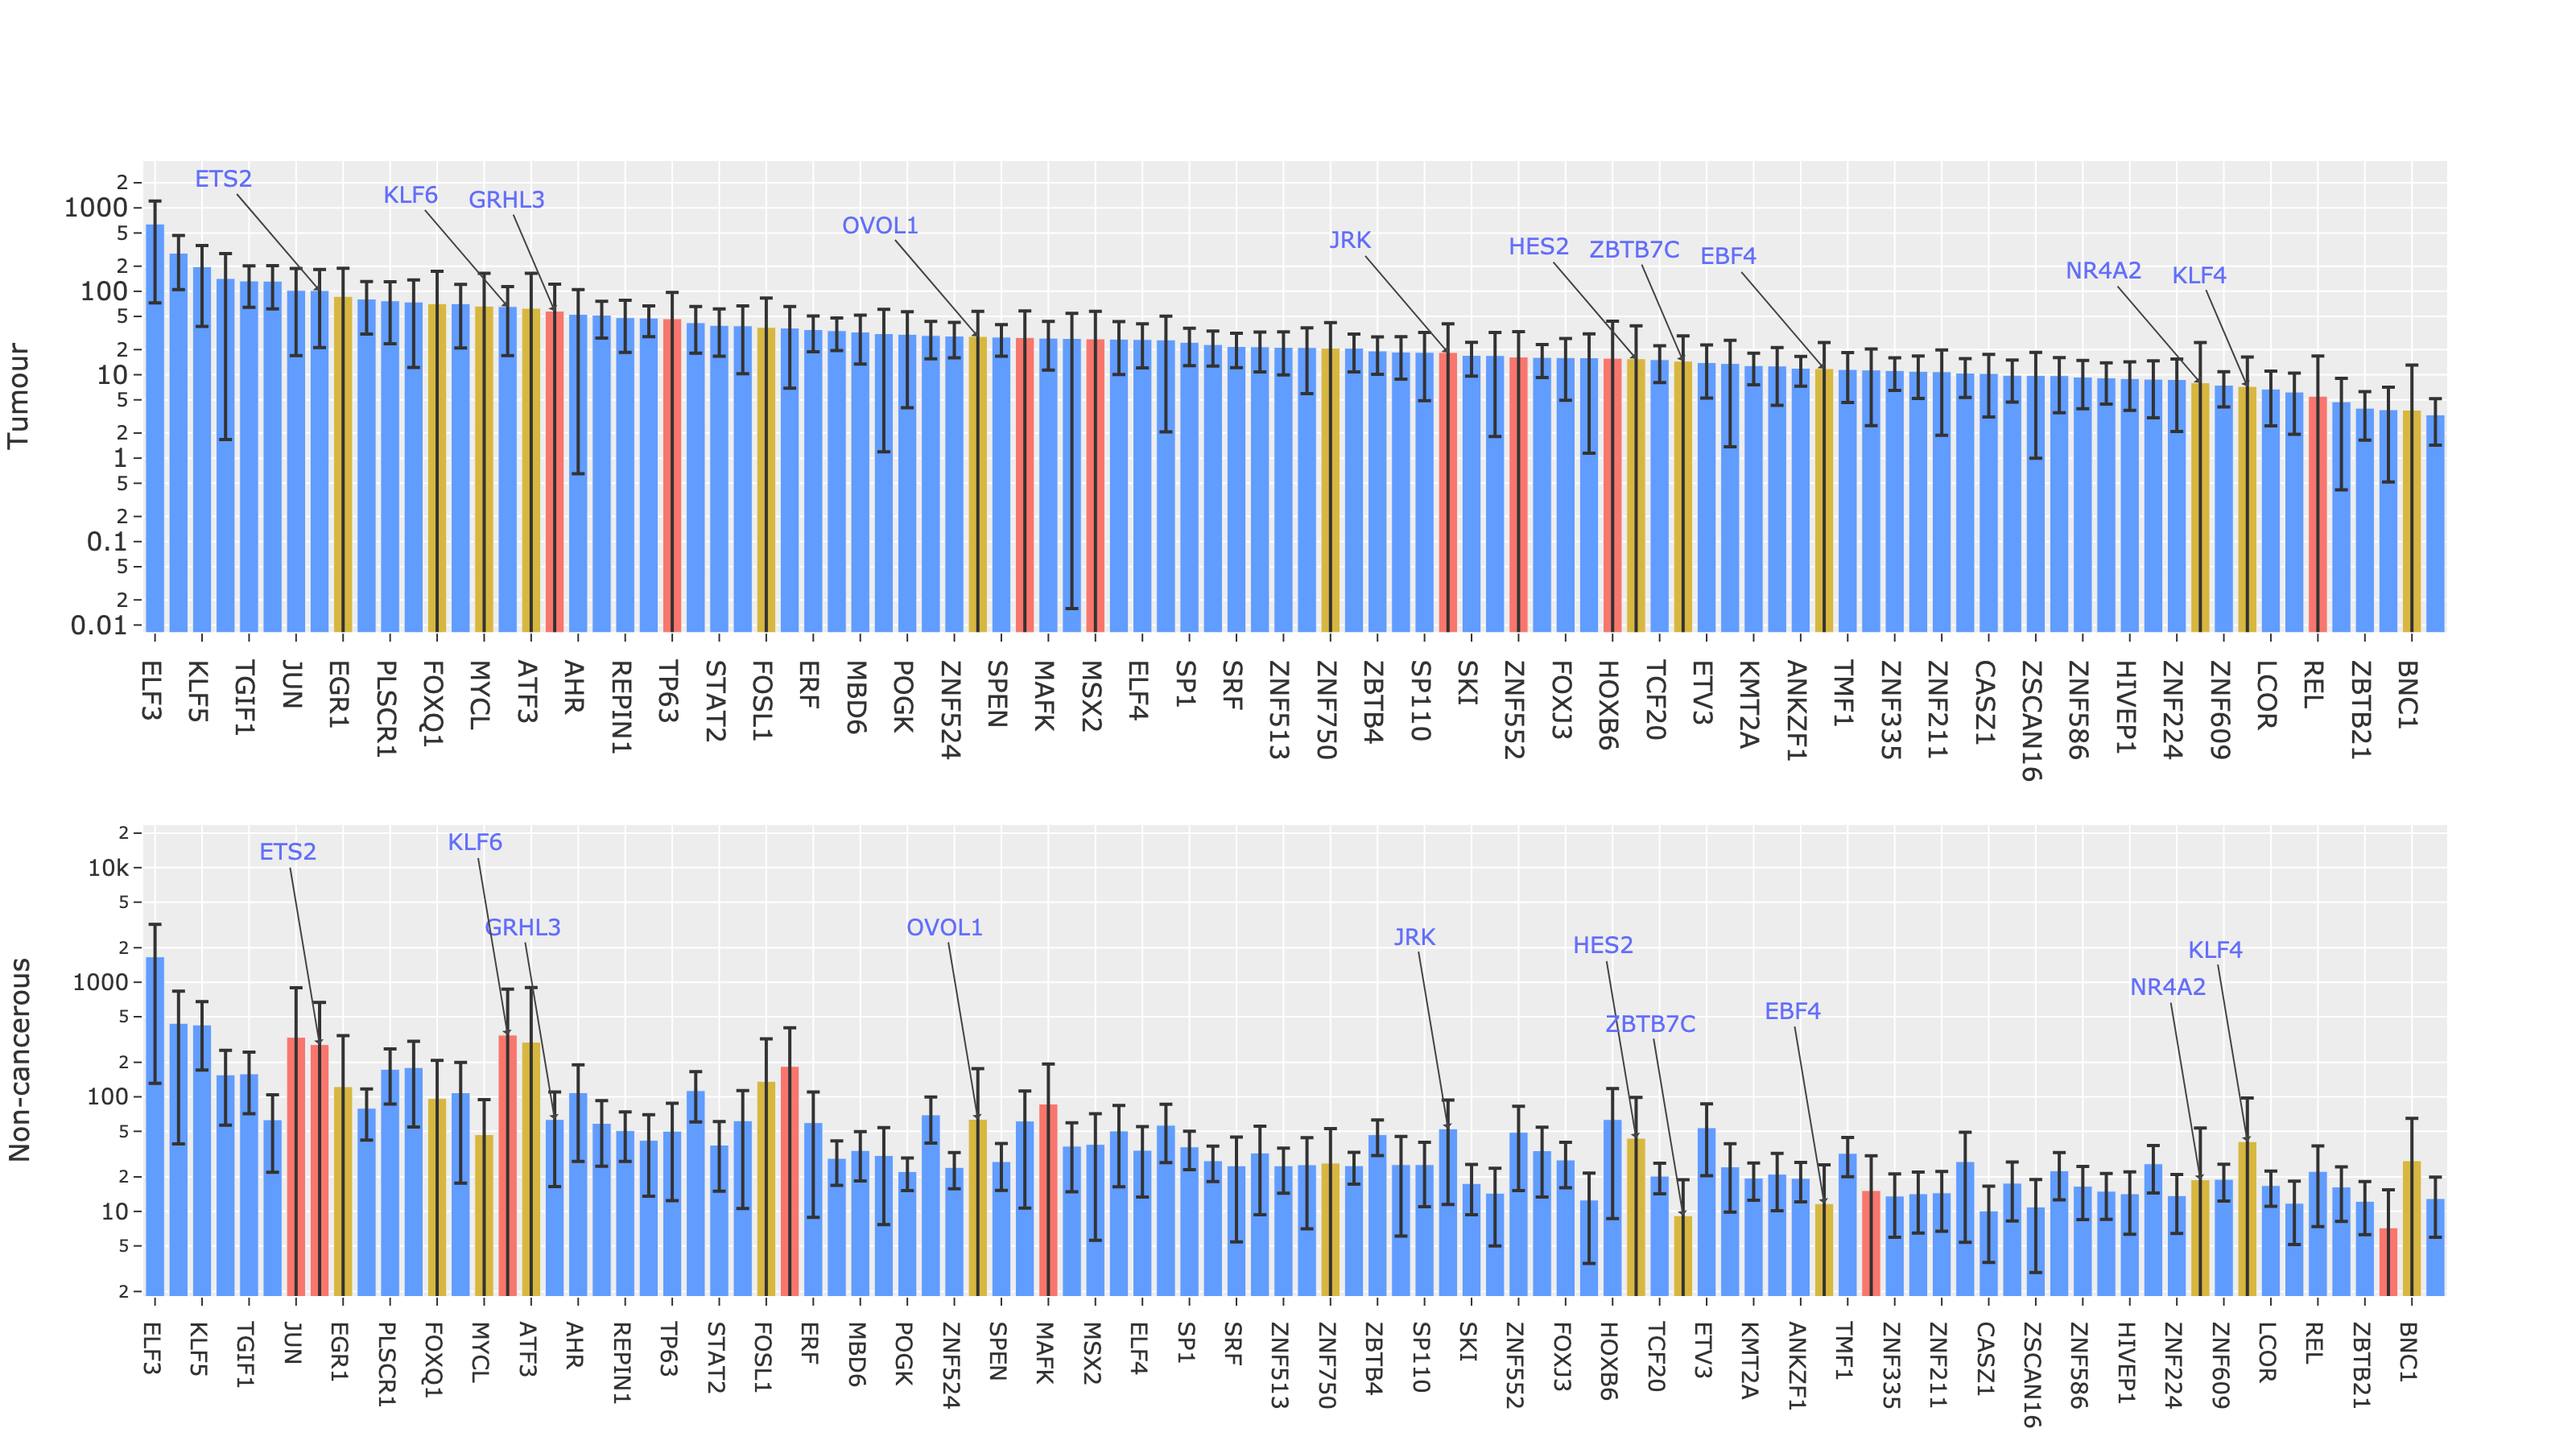
\includegraphics[width=1.0\textwidth,height=1.0\textheight,keepaspectratio]{Sections/Network_I/Resources/selective_pruning/sel_tfs/sel_tfs_var_tum_healthy.png}
  \caption{Bar plot of the log mean expression in both non-cancerous and tumour datasets with the error bars accounting for standard deviation. The genes are ordered in descending order by the mean values in the non-cancerous dataset. Red bars represents genes that have a high variance in the corresponding dataset, while the golden shows the TFs in both tumour and non-cancerous.}
\label{fig:N_I:sel_tfs_var}
\end{figure}

There are few genes that are highly expressed in both the tumours and non-cancerous datasets such as \textit{ELF3, KLF5} or \textit{JUN}. A scatter plot version of the bar plot can be seen in \cref{fig:ap:sel_tfs_mean} from Appendix, where the x-axis represents the non-cancerous mean, y-axis the tum mean and the size and colour the mutation burden of the genes.

\begin{table}[H]
  \centering
  \scriptsize
  \begin{tabularx}{\textwidth}{>{\hsize=.25\hsize}X|>{\hsize=.75\hsize}X}
    \toprule
    \textbf{Category} & \textbf{Genes} \\
    \midrule
    Varied in Both & \textit{OVOL1, FOSL1, KLF4, BNC1, MYCL, NR4A2, ZBTB7C, FOXQ1, ZNF750, EGR1, HES2, ATF3, EBF4} \\
    \midrule
    Tumours only & \textit{BHLHE41, JRK, MSX2, TP63, ZNF552, GRHL3, HOXB6, REL} \\
    \midrule
    Non-cancerous only & \textit{ZBTB10, ARID5B, KLF6, JUN, MAFF, ETS2, MAFK} \\
    \bottomrule
  \end{tabularx}
    \caption{Gene Variation Across Sample Types} % Caption for the table
    \label{tab:N_I:sel_tfs_var}
\end{table}

It is worth remembering that MIBC is generally divided into Luminal and Basal subgroups, the former exhibiting differentiated status, while the latter an undifferentiated status. The non-cancerous dataset contains samples that are either differentiated (Abs-Ca or in-situ) or undifferentiated. This implies that the TFs with a high mean deviation may play a role in differentiation and also help in understanding the Basal/Luminal differences in MIBC. The molecular particularities in the tissue types of differentiation tissues are next explored.

% Undiff vs Diff
\subsection{In bladder differentiation} \label{s:N:sel_tf_diff_status}

\begin{figure}[!h]
    \captionsetup[subfigure]{justification=Centering}
\begin{subfigure}[!t]{1.0\textwidth}
    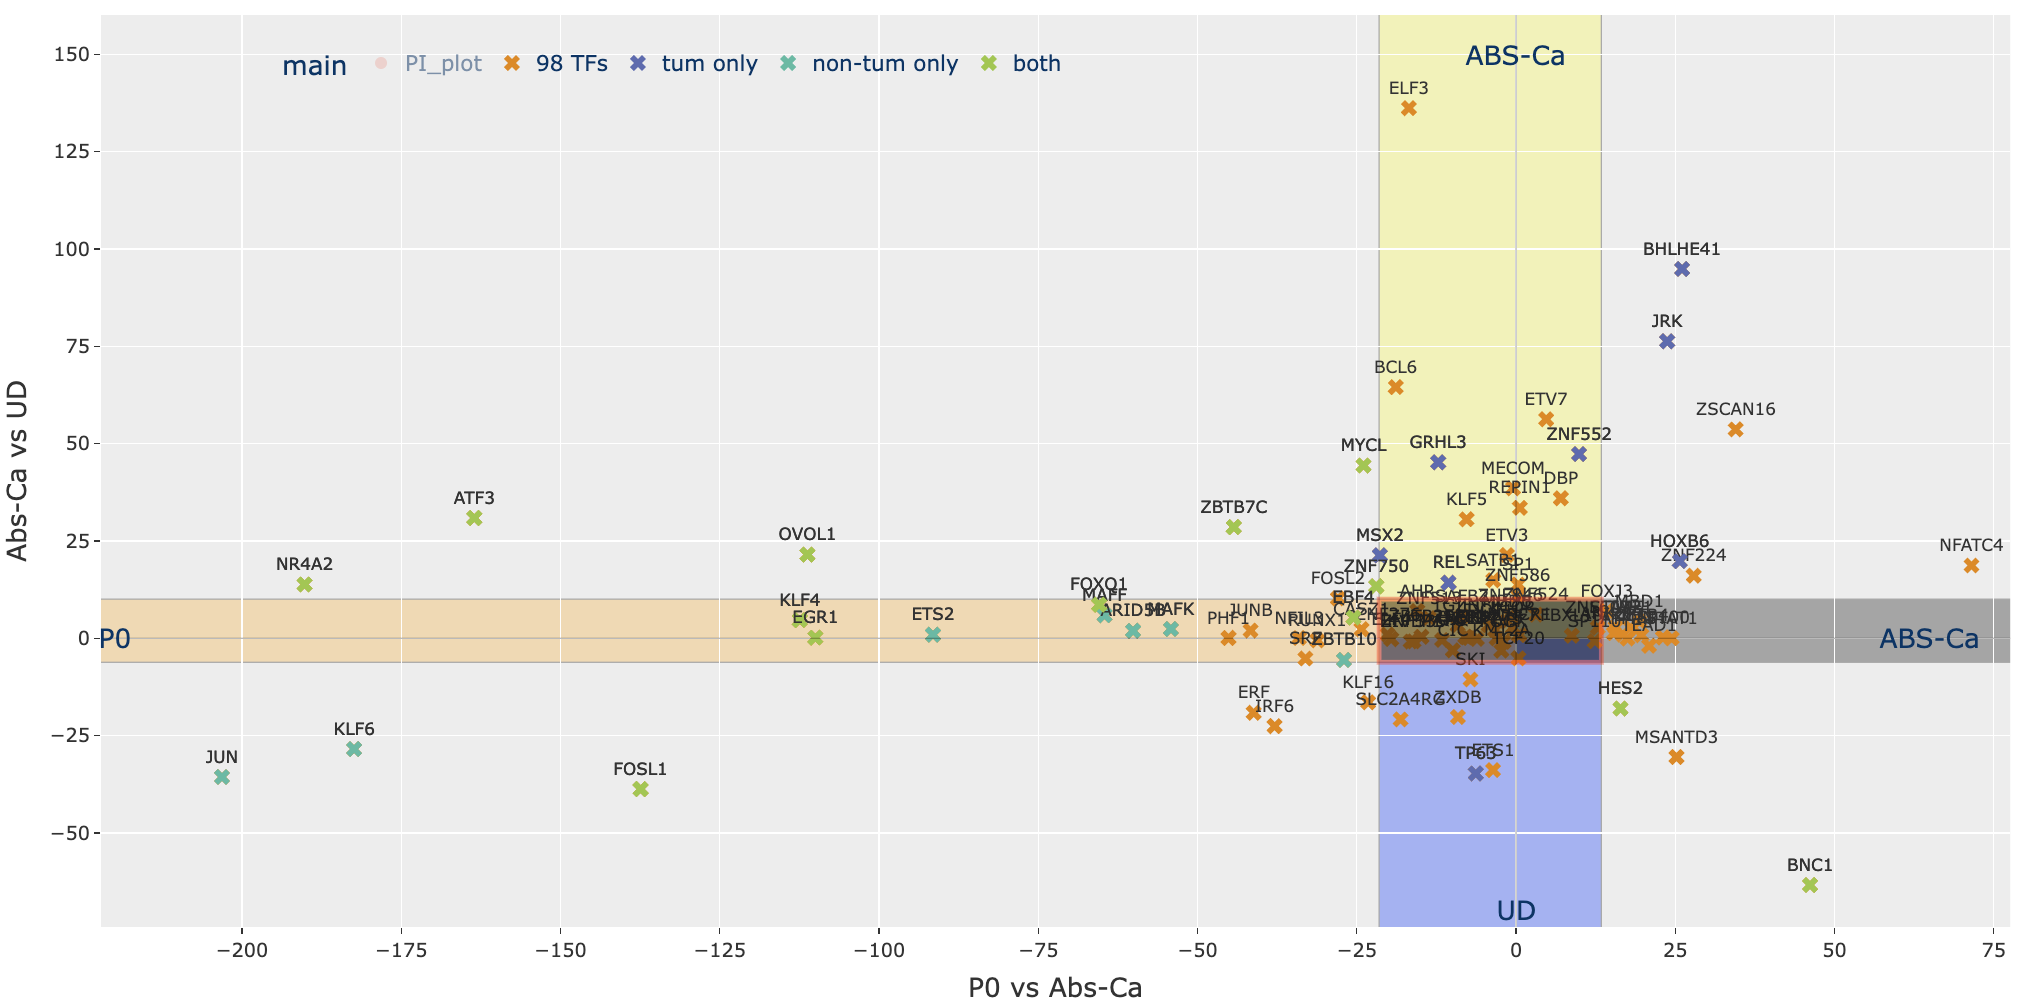
\includegraphics[width=1.0\textwidth,height=1.0\textheight,keepaspectratio]{Sections/Network_I/Resources/selective_pruning/sel_tfs/sel_tfs_pi_all_var_rect.png}
    
    \caption{Pi plot with just the varied genes}
    
    \label{fig:N_I:pi_sel_tfs_var}
\end{subfigure}\hspace{\fill} % maximize horizontal separation

\begin{subfigure}[!t]{1.0\textwidth}
    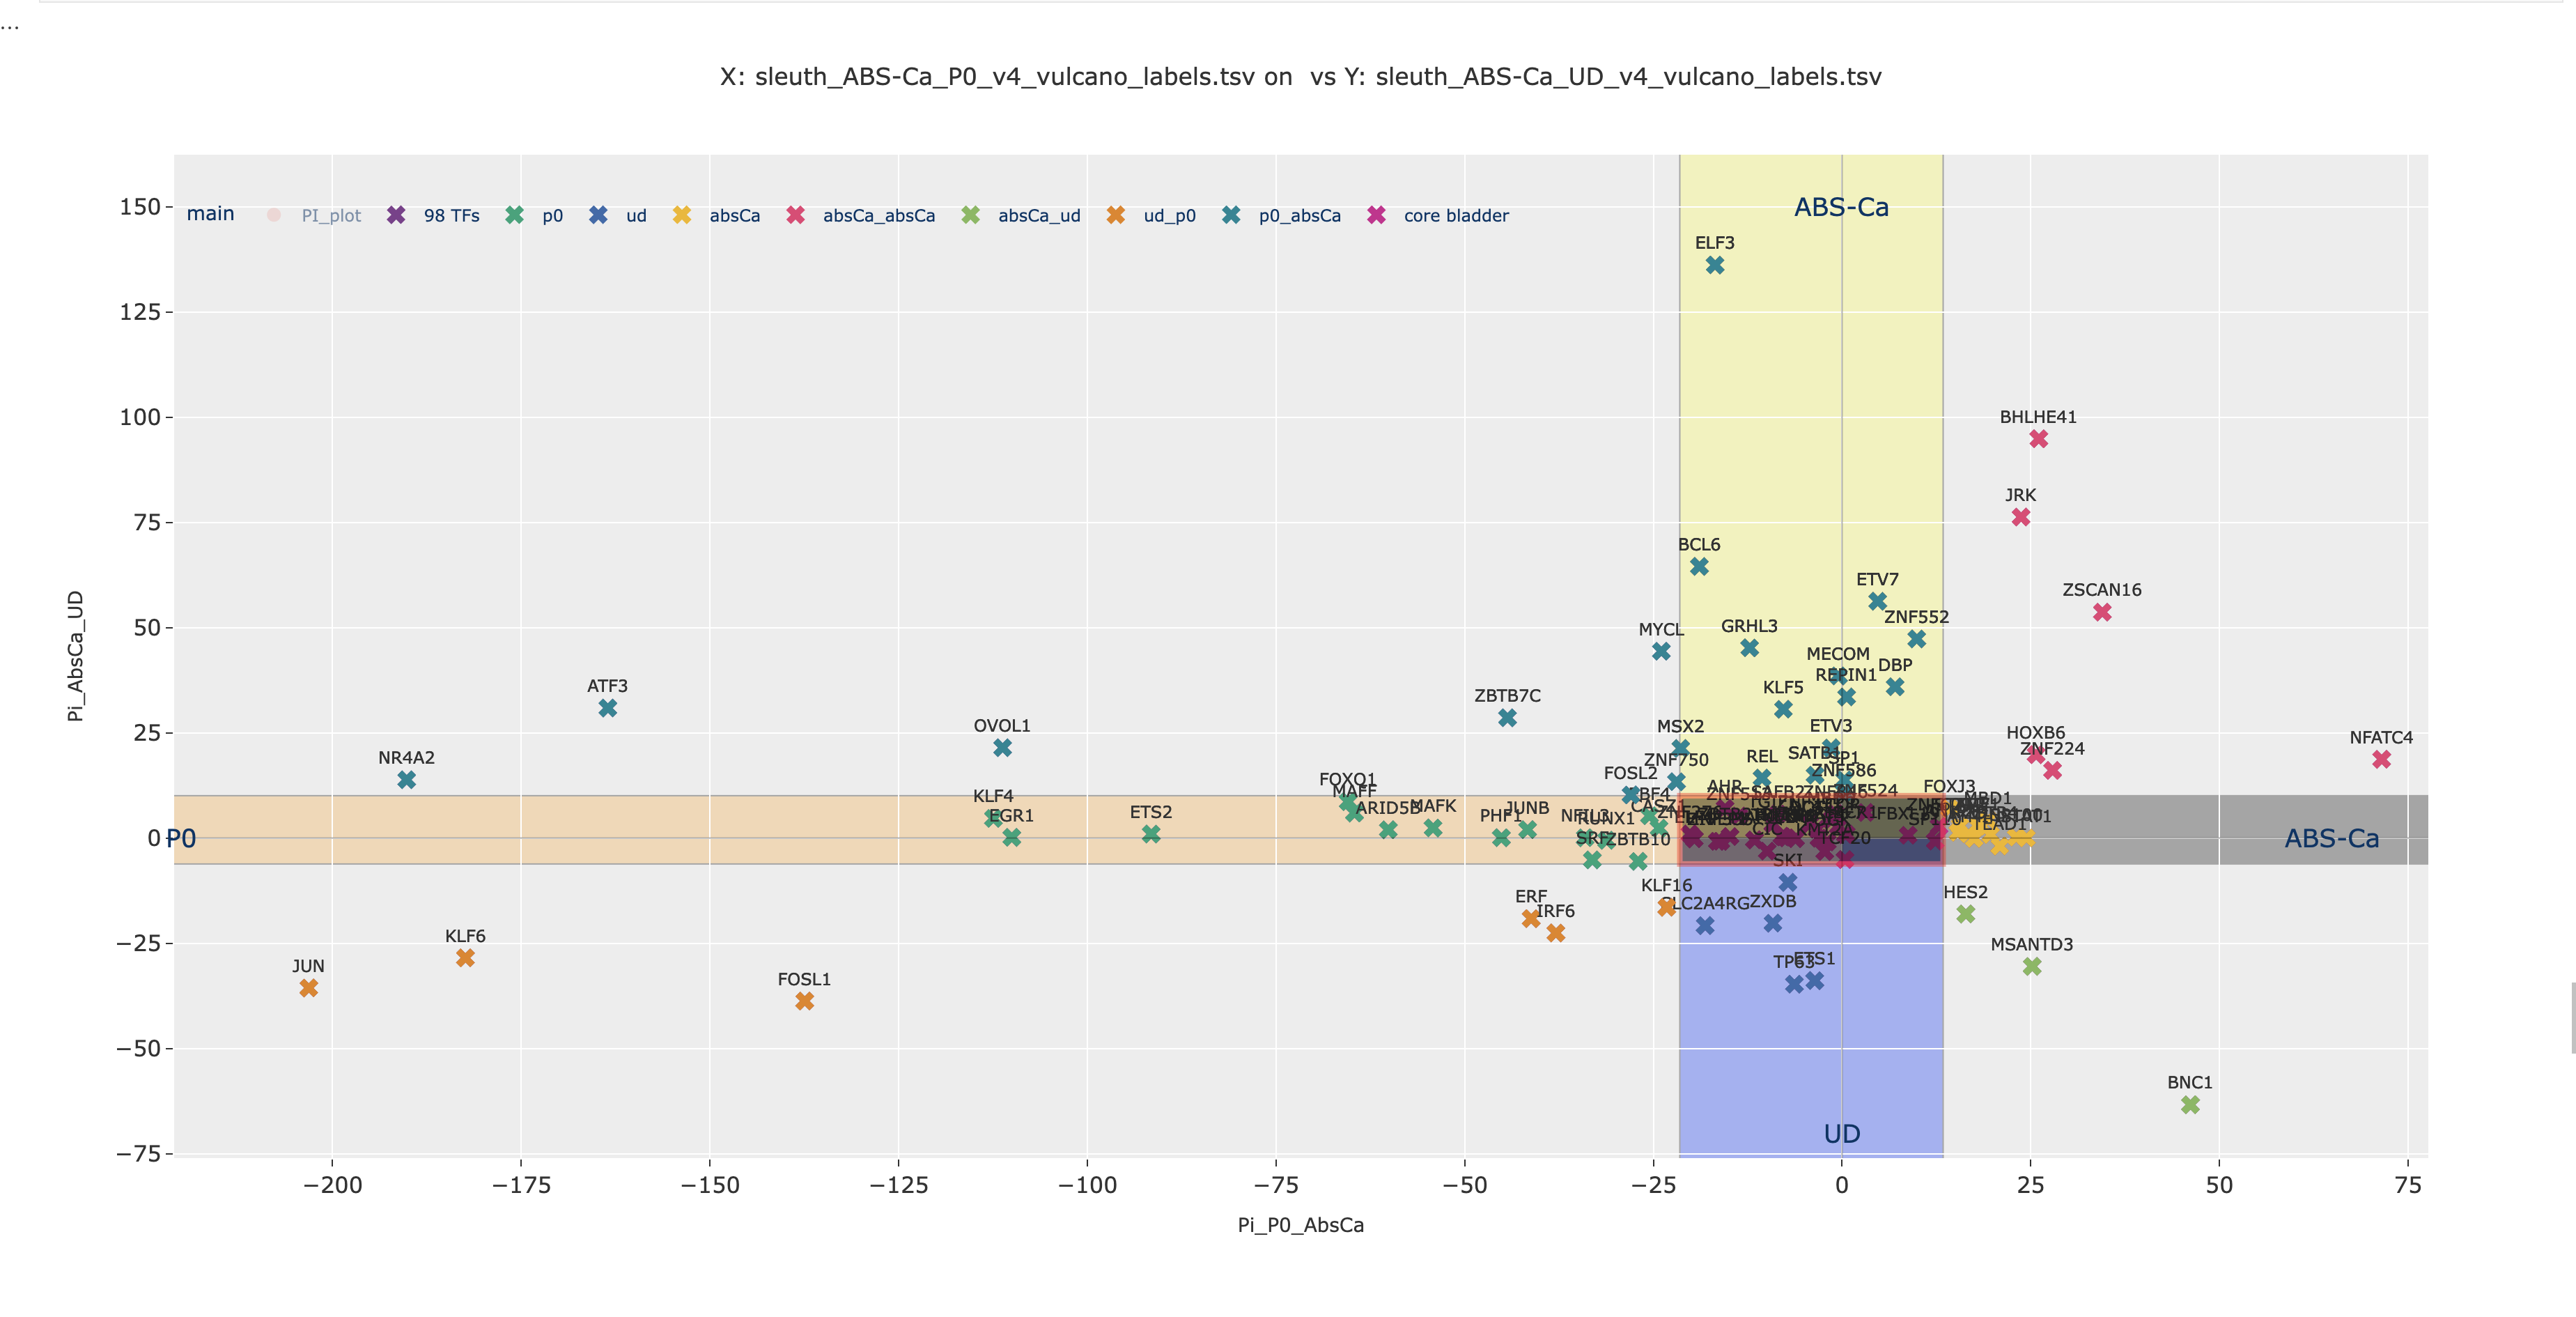
\includegraphics[width=1.0\textwidth,height=1.0\textheight,keepaspectratio]{Sections/Network_I/Resources/selective_pruning/sel_tfs/sel_tfs_pi_all_tissueDiff.png}
    
    \caption{Pi plot with all the 98 TFs}
    
    \label{fig:N_I:pi_sel_tfs_all}
\end{subfigure}\hspace{\fill} % maximize horizontal separation

    \caption{Two Pi plots of the same comparisons, but with different markers shown. The X-axis represents the Pi values from the DEA of the P0 vs AbsCa, the Y-axis from AbsCa vs UD. The markers yellow are the most varied genes seen in \cref{fig:N_I:sel_tfs_var}, the blue the genes highly varied only in the non-cancerous where the green highly varied in the tumour. The rest of the markers in purple are rest of the 98 TFs gene.}
    
    \label{fig:N_I:pi_sel_tfs}
\end{figure}

% Introducing the two pi-plots
The pi plot in \cref{fig:N_I:pi_sel_tfs} presents the 98 TFs in the context of the non-cancerous tumour dataset from the JBU. The Y coordinate is given by the pi value (-$log10(q)*fold\_change$) from the DEA performed between the Undifferentiated (UD) and Abs-Calcium (AbsCa) group, where the X-coordinate is the comparison between AbsCa and P0 (in-situ). The positive values on the Y-axis represents the ABS-Ca specific TF, while the negative values the genes closed to UD. Where the negative values on the X-axis are P0 specific and conversely for the positive values and AbsCa. The rectangles are drawn  within $+/-5\%$ of the axes and are a visual cue for the genes that are very close to the axis. These are different scales as the pi values across comparison has different ranges. This difference in axes ranges needs to be accounted for when interpreting the plot, especially in the UD - P0 quadrant. 

% Just the sel tfs - UD and P0
In \cref{fig:N_I:pi_sel_tfs}, it can be seen that \textit{BNC1} and \textit{HES2} are UD markers, which may also indicate specificity for squamous markers. \textit{TP63} is another squamous marker \cite{Robertson2017-mg}, but it is more significantly differentiated in the UD vs Abs-Ca comparison. \textit{FOSL1} is a highly varied gene that appears to be both an undifferentiated and P0 marker (note the difference in scale between the X-axis and Y-axis). \textit{KLF6} and \textit{JUN} are genes more specific to P0 but are also highly expressed in the undifferentiated tissue.


% Talk about the differentiation markers 
The two Y-positive quadrants contains the genes that are likely involved in the differentiation of the bladder tissue, closer to the x-axis, more specific to the culture mode, conversely to Y-axis to the P0. It is worth noting that most of the genes specific to Abs-Ca model are highly varied in the tumours, which may suggest that are more expressed in the Luminal tumours compared to the Basal; \textit{HOXB6, ZNF552, JRK, BHLHe41}. Genes \textit{ZNF750, MSX2, MYCL, GRHL3 and REL} are specific to both P0 and Abs-Ca. Both \textit{MYCL, GRHL3} are known to be differentiation markers. There are also markers that are specific to P0 samples: \textit{EBF4, MAFK, ARID5B, EGR1, ETS2, MAFF, FOX1, KLF4, NR4A2, ATF3, OVOL1}. 

While \cref{fig:N_I:pi_sel_tfs_var} offer a focused view on the TFs that are varied in the non-cancerous and/or the MIBC cohort from TCGA, \cref{fig:N_I:pi_sel_tfs_all} complements the plot by showing all the 98 TFs. It can be noticed that there are several markers that might be UD specific (negative X-axis) while some additional markers involved in differentiation which do not vary as much. The latter may suggest that these markers are common both in Basal and Luminal tumours. 

% No TFs shared between UD and Abs-Ca
It is surprising that there are no TFs shared in the culture quadrant (UD and Abs-Ca) and many TFs in the middle of the Pi plot. The genes at the centre of the pi plot may indicate a list of TFs that are at the core of bladder tissue, regardless if it is differentiated or undifferentiated.

\begin{table}[H]
  \centering
  \scriptsize
  \begin{tabularx}{\textwidth}{>{\hsize=.15\hsize}X|>{\hsize=.85\hsize}X}
    \toprule
    \textbf{Category} & \textbf{Genes} \\
    \midrule
    \textbf{P0} & \textit{KLF4, ETS2, PHF1, ARID5B, EGR1, FOXQ1, MAFF, JUNB, MAFK, NFIL3, SRF, RUNX1, CASZ1, ZBTB10, EBF4} \\
    \midrule
    \textbf{UD} & \textit{SLC2A4RG, ZXDB, SKI, TP63, ETS1} \\
    \midrule
    \textbf{AbsCa} & \textit{BCL6, MSX2, ELF3, GRHL3, REL, KLF5, ZNF552, SATB1, DBP, ETV7, ETV3, MECOM, REPIN1, SP1, ZNF586, ZBTB4, TEAD1, ATMIN, TMF1, SP100, FOXJ3, MBD1, STAT1, ANKZF1, IRF9, STAT2, NFATC4, ZNF224, ZSCAN16, JRK, BHLHE41, HOXB6} \\
    \midrule
    \textbf{AbsCa-UD} & \textit{BNC1, MSANTD3, HES2} \\
    \midrule
    \textbf{UD-P0} & \textit{KLF6, JUN, FOSL1, ERF, IRF6, KLF16} \\
    \midrule
    \textbf{P0-AbsCa} & \textit{NR4A2, ATF3, OVOL1, ZBTB7C, FOSL2, BCL6, MSX2, MYCL, ZNF750, ELF3, GRHL3, REL, KLF5, ZNF552, SATB1, DBP, ETV7, ETV3, MECOM, REPIN1, SP1, ZNF586} \\
    \bottomrule
  \end{tabularx}
  \caption{TF marker classified by being significantly expressed in the two DEA comparisons: P0 vs AbsCa and UD vs AbsCa in \cref{fig:N_I:pi_sel_tfs}.} 
  \label{tab:N_I:markers_diff}
\end{table}

\Cref{tab:N_I:markers_diff} summarises the TF classification based on the differentiation tissue type: AbsCa (differentiation in culture), P0 (differentiation in tissue) and undifferentiated (culture). The 'transitional' genes in AbsCa-UD, UD-P0 and P0-AbsCa may yield information about the common genes shared between differentiation tissue types.


% Transitioning to cancer
\subsection{In muscle-invasive bladder cancer} \label{s:N_I:sel_tfs_cancer}


% Selecting the genes for basal and luminal, expression in both Basal and Luminal
Using the above work and the box plots like the ones in \cref{fig:N_I:box_basal,fig:N_I:box_luminal}, two lists of genes specific to Basal/Squamous (Ba/Sq) and Luminal subtypes were created, as shown in \cref{tab:N_I:genes_lum_basal}. A recent study by \citet{Ramal2024-ha}, which investigated the regulatory network in urothelial cells, concluded that the following genes are considered 'novel putative TFs' for luminal differentiation: \textit{\textbf{BHLHE41}, \textbf{MECOM}, \textbf{MYCL}, NCOA1, NR2F2, NR2F6, \textbf{REPIN1}, SREBF1, TBX2, TBX3, TRAFD1, and \textbf{ZBTB7C}}. The bold genes are among the 98 TFs identified in this section, while \textit{MECOM, BHLHE41, ZBTB7C} are selected as markers in \cref{tab:N_I:genes_lum_basal}. \textit{GRHL3} is also mentioned in the work by \citet{Ramal2024-ha}, but it has already been determined as a differentiation marker \citet{Bock2014-zy}. \citet{Chen2021-tc} studied the role of \textit{ZBTB7C} across different cancers and its relation to tumour mutational burden, microsatellite instability, and immune cell infiltration.

% Lum-basal markers
\begin{table}[!htb]
  \centering
  \scriptsize
  \begin{tabularx}{\textwidth}{>{\hsize=.25\hsize}X|>{\hsize=.75\hsize}X}
    \toprule
    \textbf{Category} & \textbf{Genes} \\
    \midrule
    \textbf{Luminal} & \textit{MSX2, HOXB6, MECOM, GRHL3, JRK, BHLHE41, ZBTB7C, ZSCAN16, ZNF224, ZBTB10} \\
    \midrule
    \textbf{Basal/Squamous} & \textit{TP63, BNC1, HES2, ERF, IRF6, ZXDB, ZNF750, ETS1, MSANTD3, FOSL1, KLF6, KLF16} \\
    \bottomrule
  \end{tabularx}
  \caption{The 98 transcription factors markers categorised by Luminal and Basal subtypes.} % Caption for the table
  \label{tab:N_I:genes_lum_basal}
\end{table}

% Discuss Squamous work
\citet{Hurst2022-sp} researched the upregulated and downregulated genes involved in the formation of squamous cell carcinoma (SCC), an undifferentiated tissue. Figure 4 from their paper shows the signature genes involved in this process. Among the upregulated genes in \citet{Hurst2022-sp}, the following are found in the 98 TFs: \textit{\textbf{BNC1}, EGR1, \textbf{FOSL1}, \textbf{HES2}, JUN, \textbf{KLF16}, KLF4, NFIL3}. From the list of downregulated genes, the following are found in the 98 TFs: \textit{\textbf{BHLHE41}, ELF3, FOXQ1, \textbf{MECOM}, POGK, REPIN1, ZSCAN16}. The bold genes are the markers chosen as markers for basal and luminal (\cref{tab:N_I:genes_lum_basal}).


% % Basal Markers 
\begin{figure}[H]
    \captionsetup[subfigure]{justification=Centering}
    % consensus
    \begin{subfigure}[!t]{0.49\textwidth}
        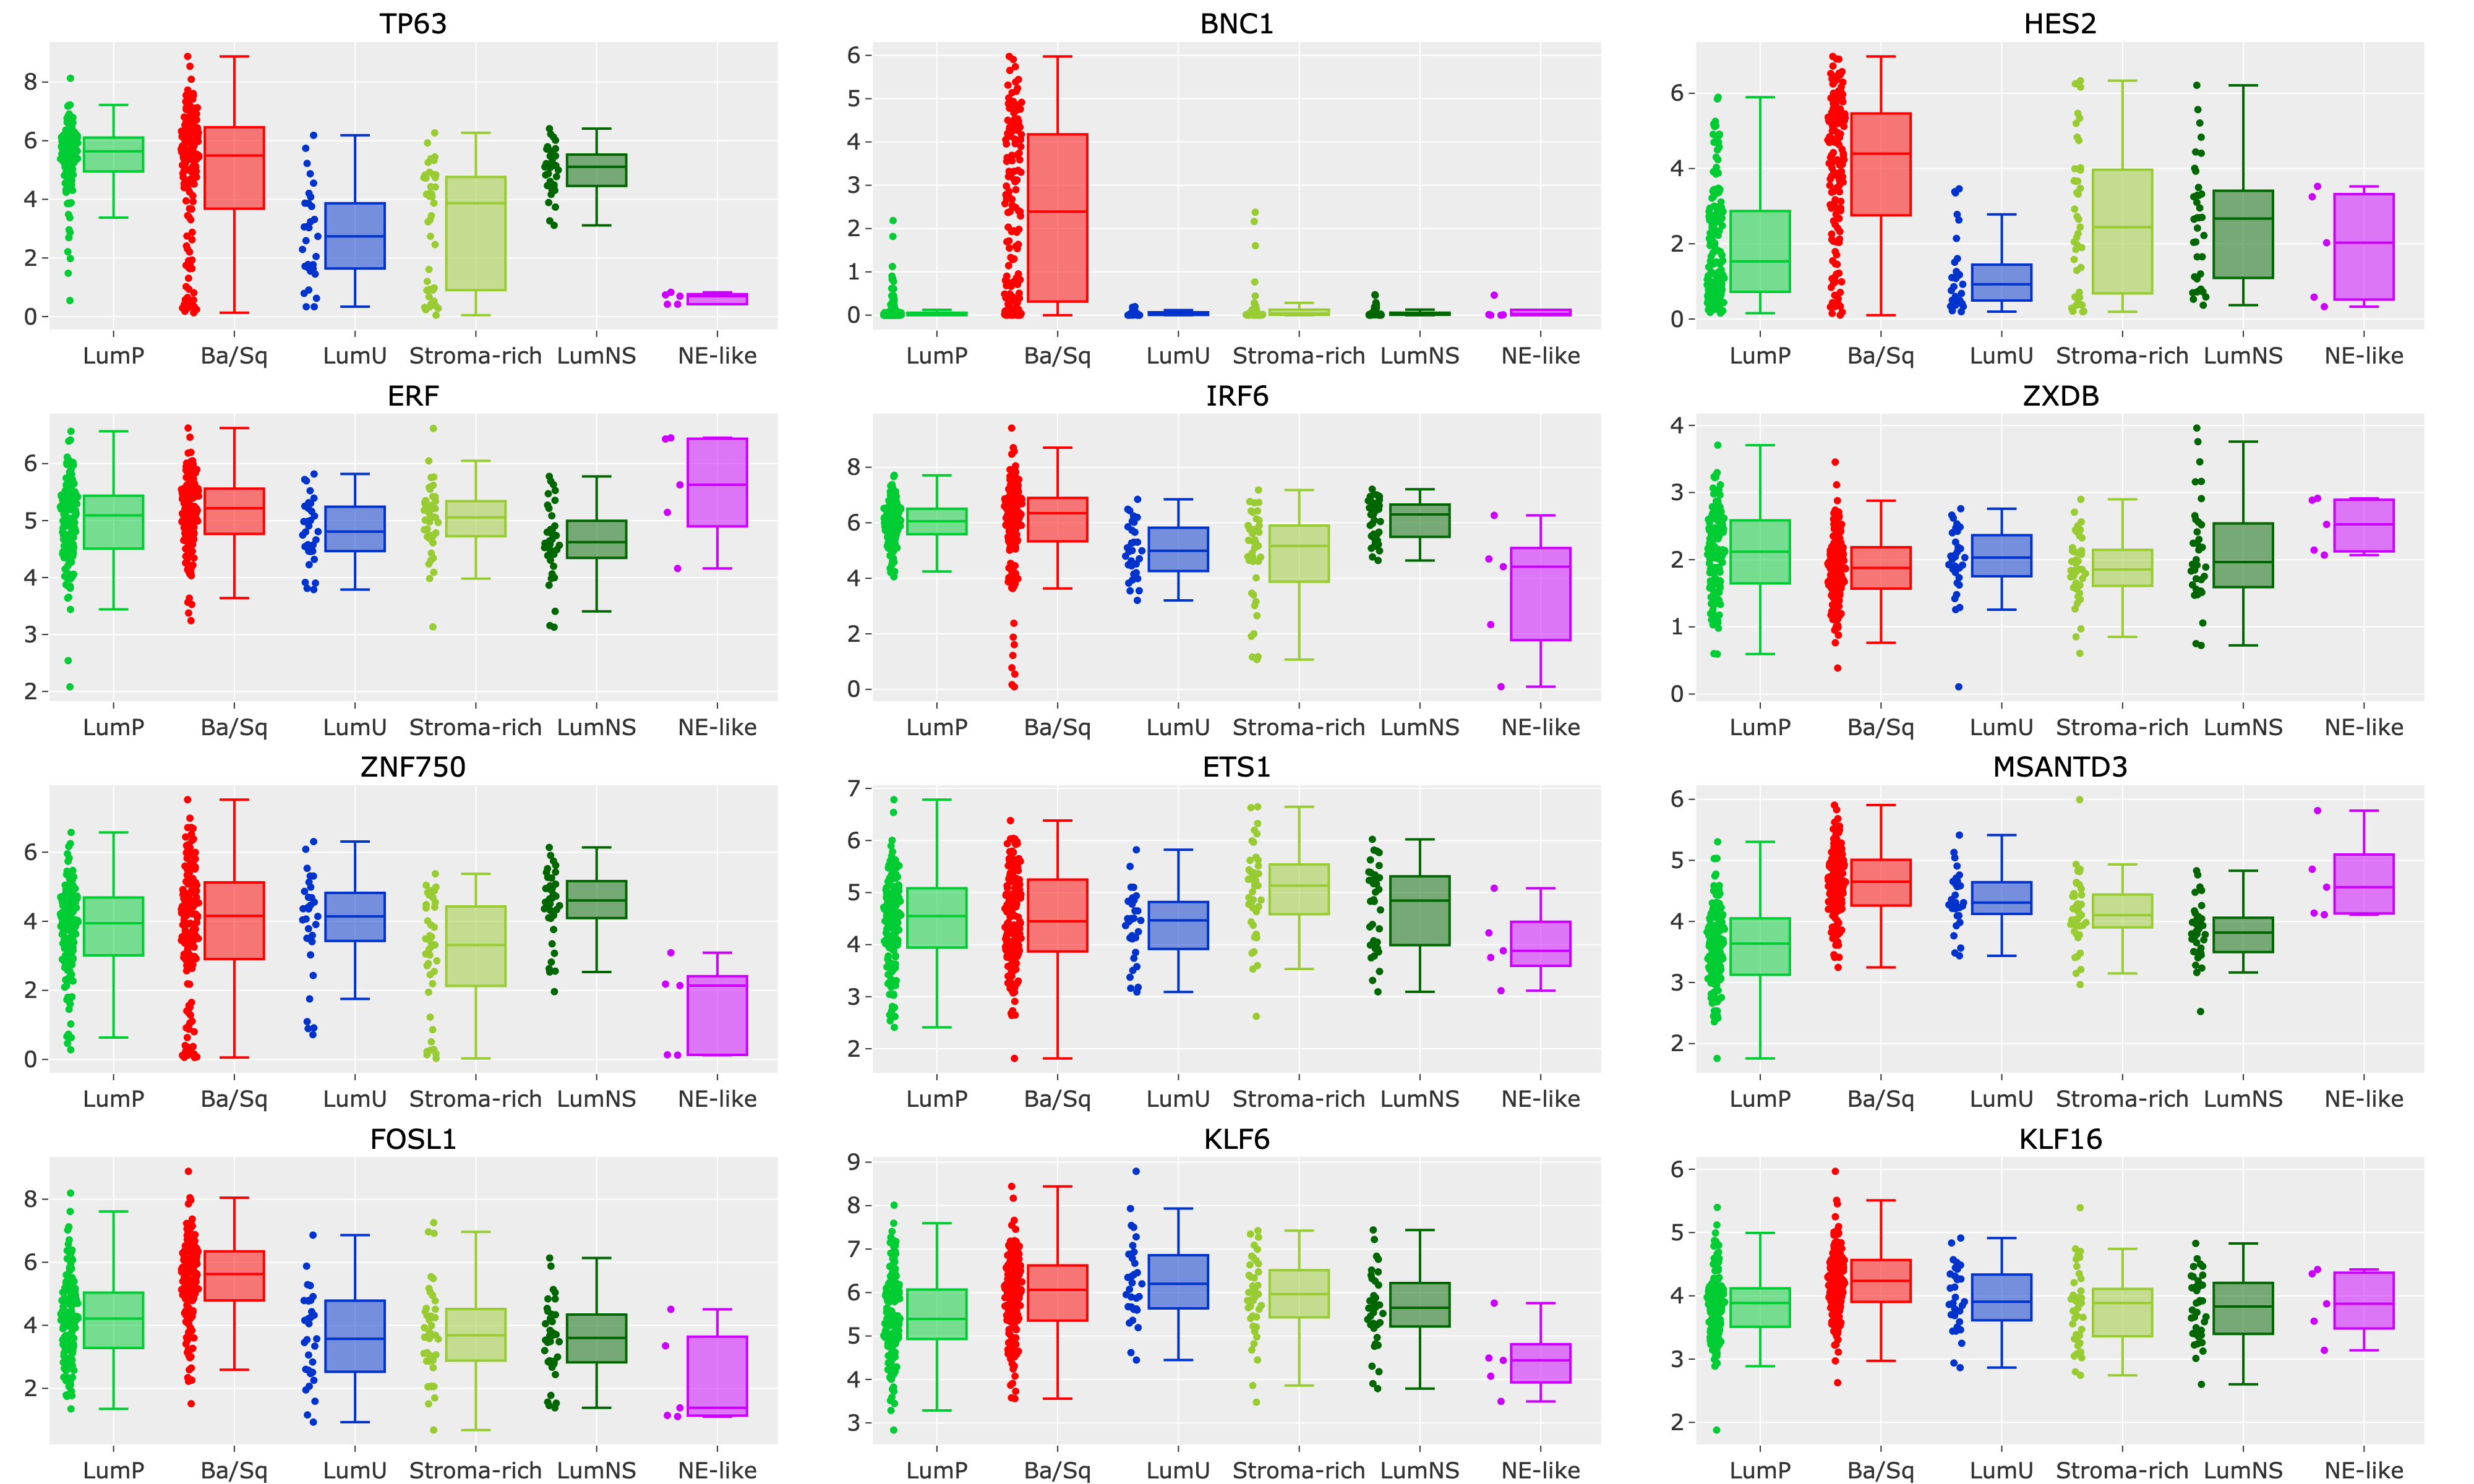
\includegraphics[width=1.0\textwidth,height=1.0\textheight,keepaspectratio]{Sections/Network_I/Resources/selective_pruning/log2_consensus_basal.png}
        \caption{Consensus}
        \label{fig:N_I:box_basal_consensus}
    \end{subfigure}
    \begin{subfigure}[!t]{0.49\textwidth}
        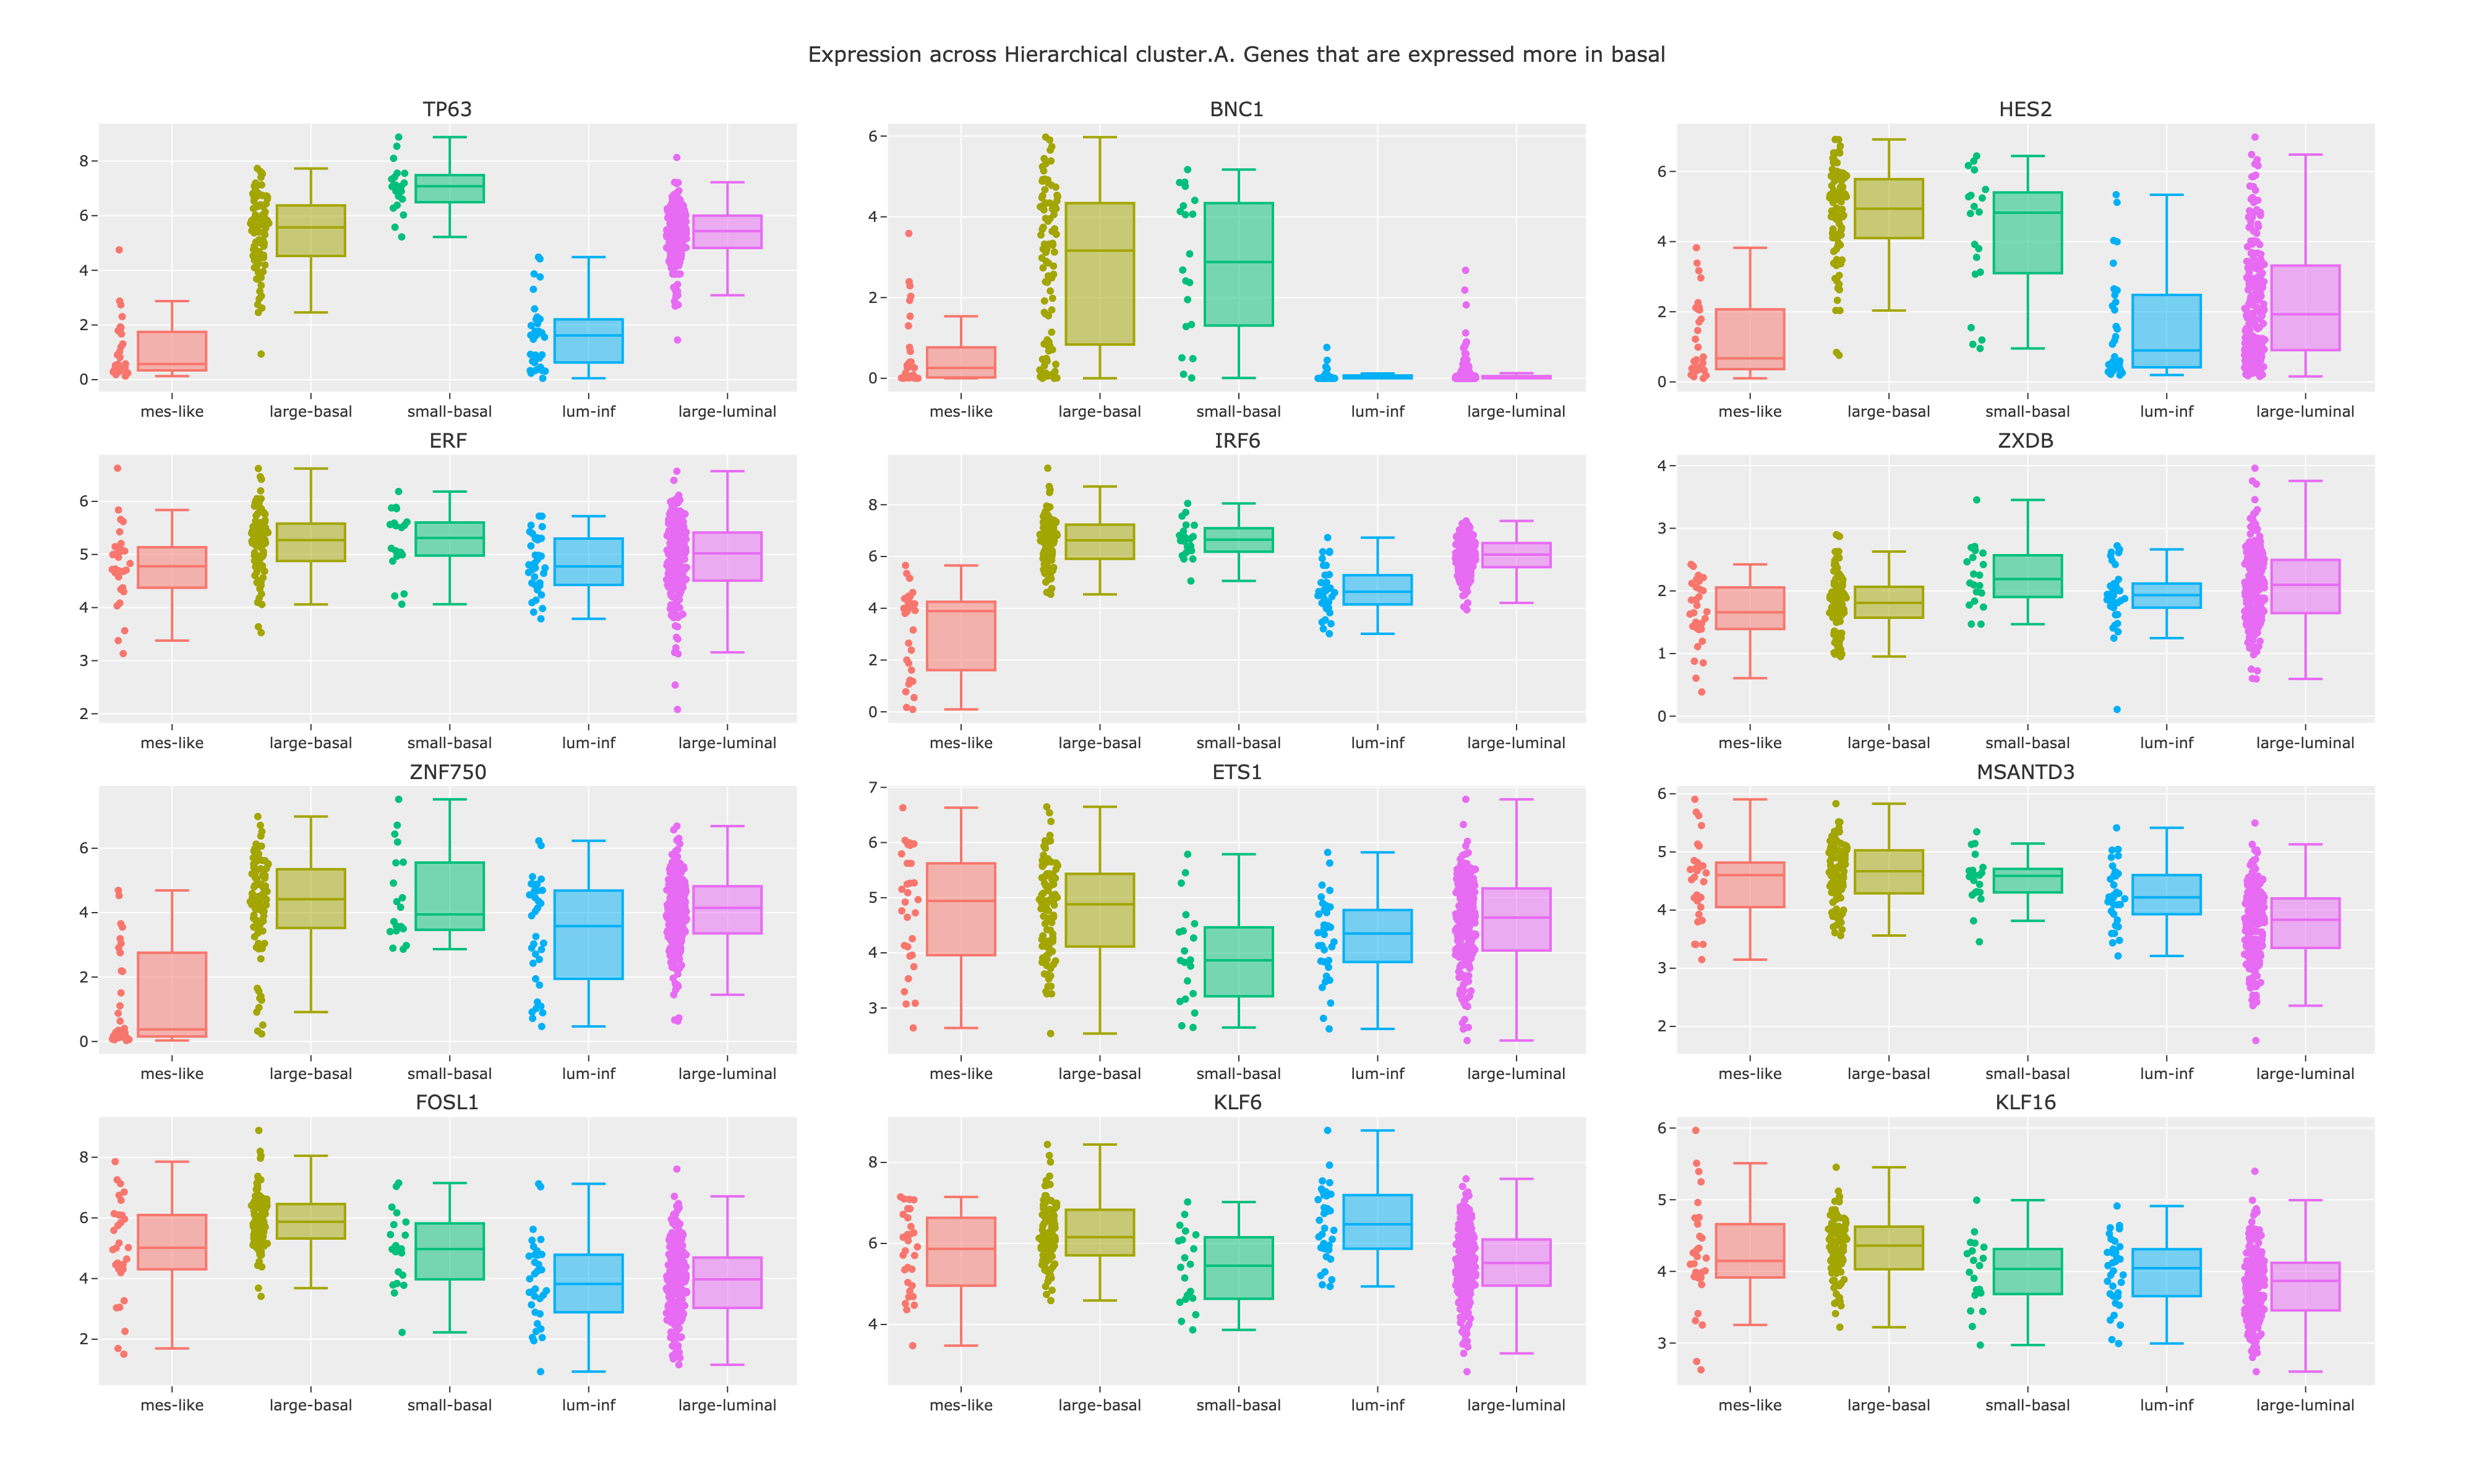
\includegraphics[width=1.0\textwidth,height=1.0\textheight,keepaspectratio]{Sections/Network_I/Resources/selective_pruning/log2_dendrogram_basla.png}
        \caption{Basal}
        \label{fig:N_I:box_basal_dendrogram}
    \end{subfigure}
    \caption{Box plots showing the $log2(TPM+1)$ of the \textbf{basal} markers over the consensus and groups derived from the hierarchical clustering applied in this chapter.}
    \label{fig:N_I:box_basal}
\end{figure}



% \begin{sidewaysfigure}
%   \centering
%     \begin{subfigure}[!t]{0.49\textwidth}
%      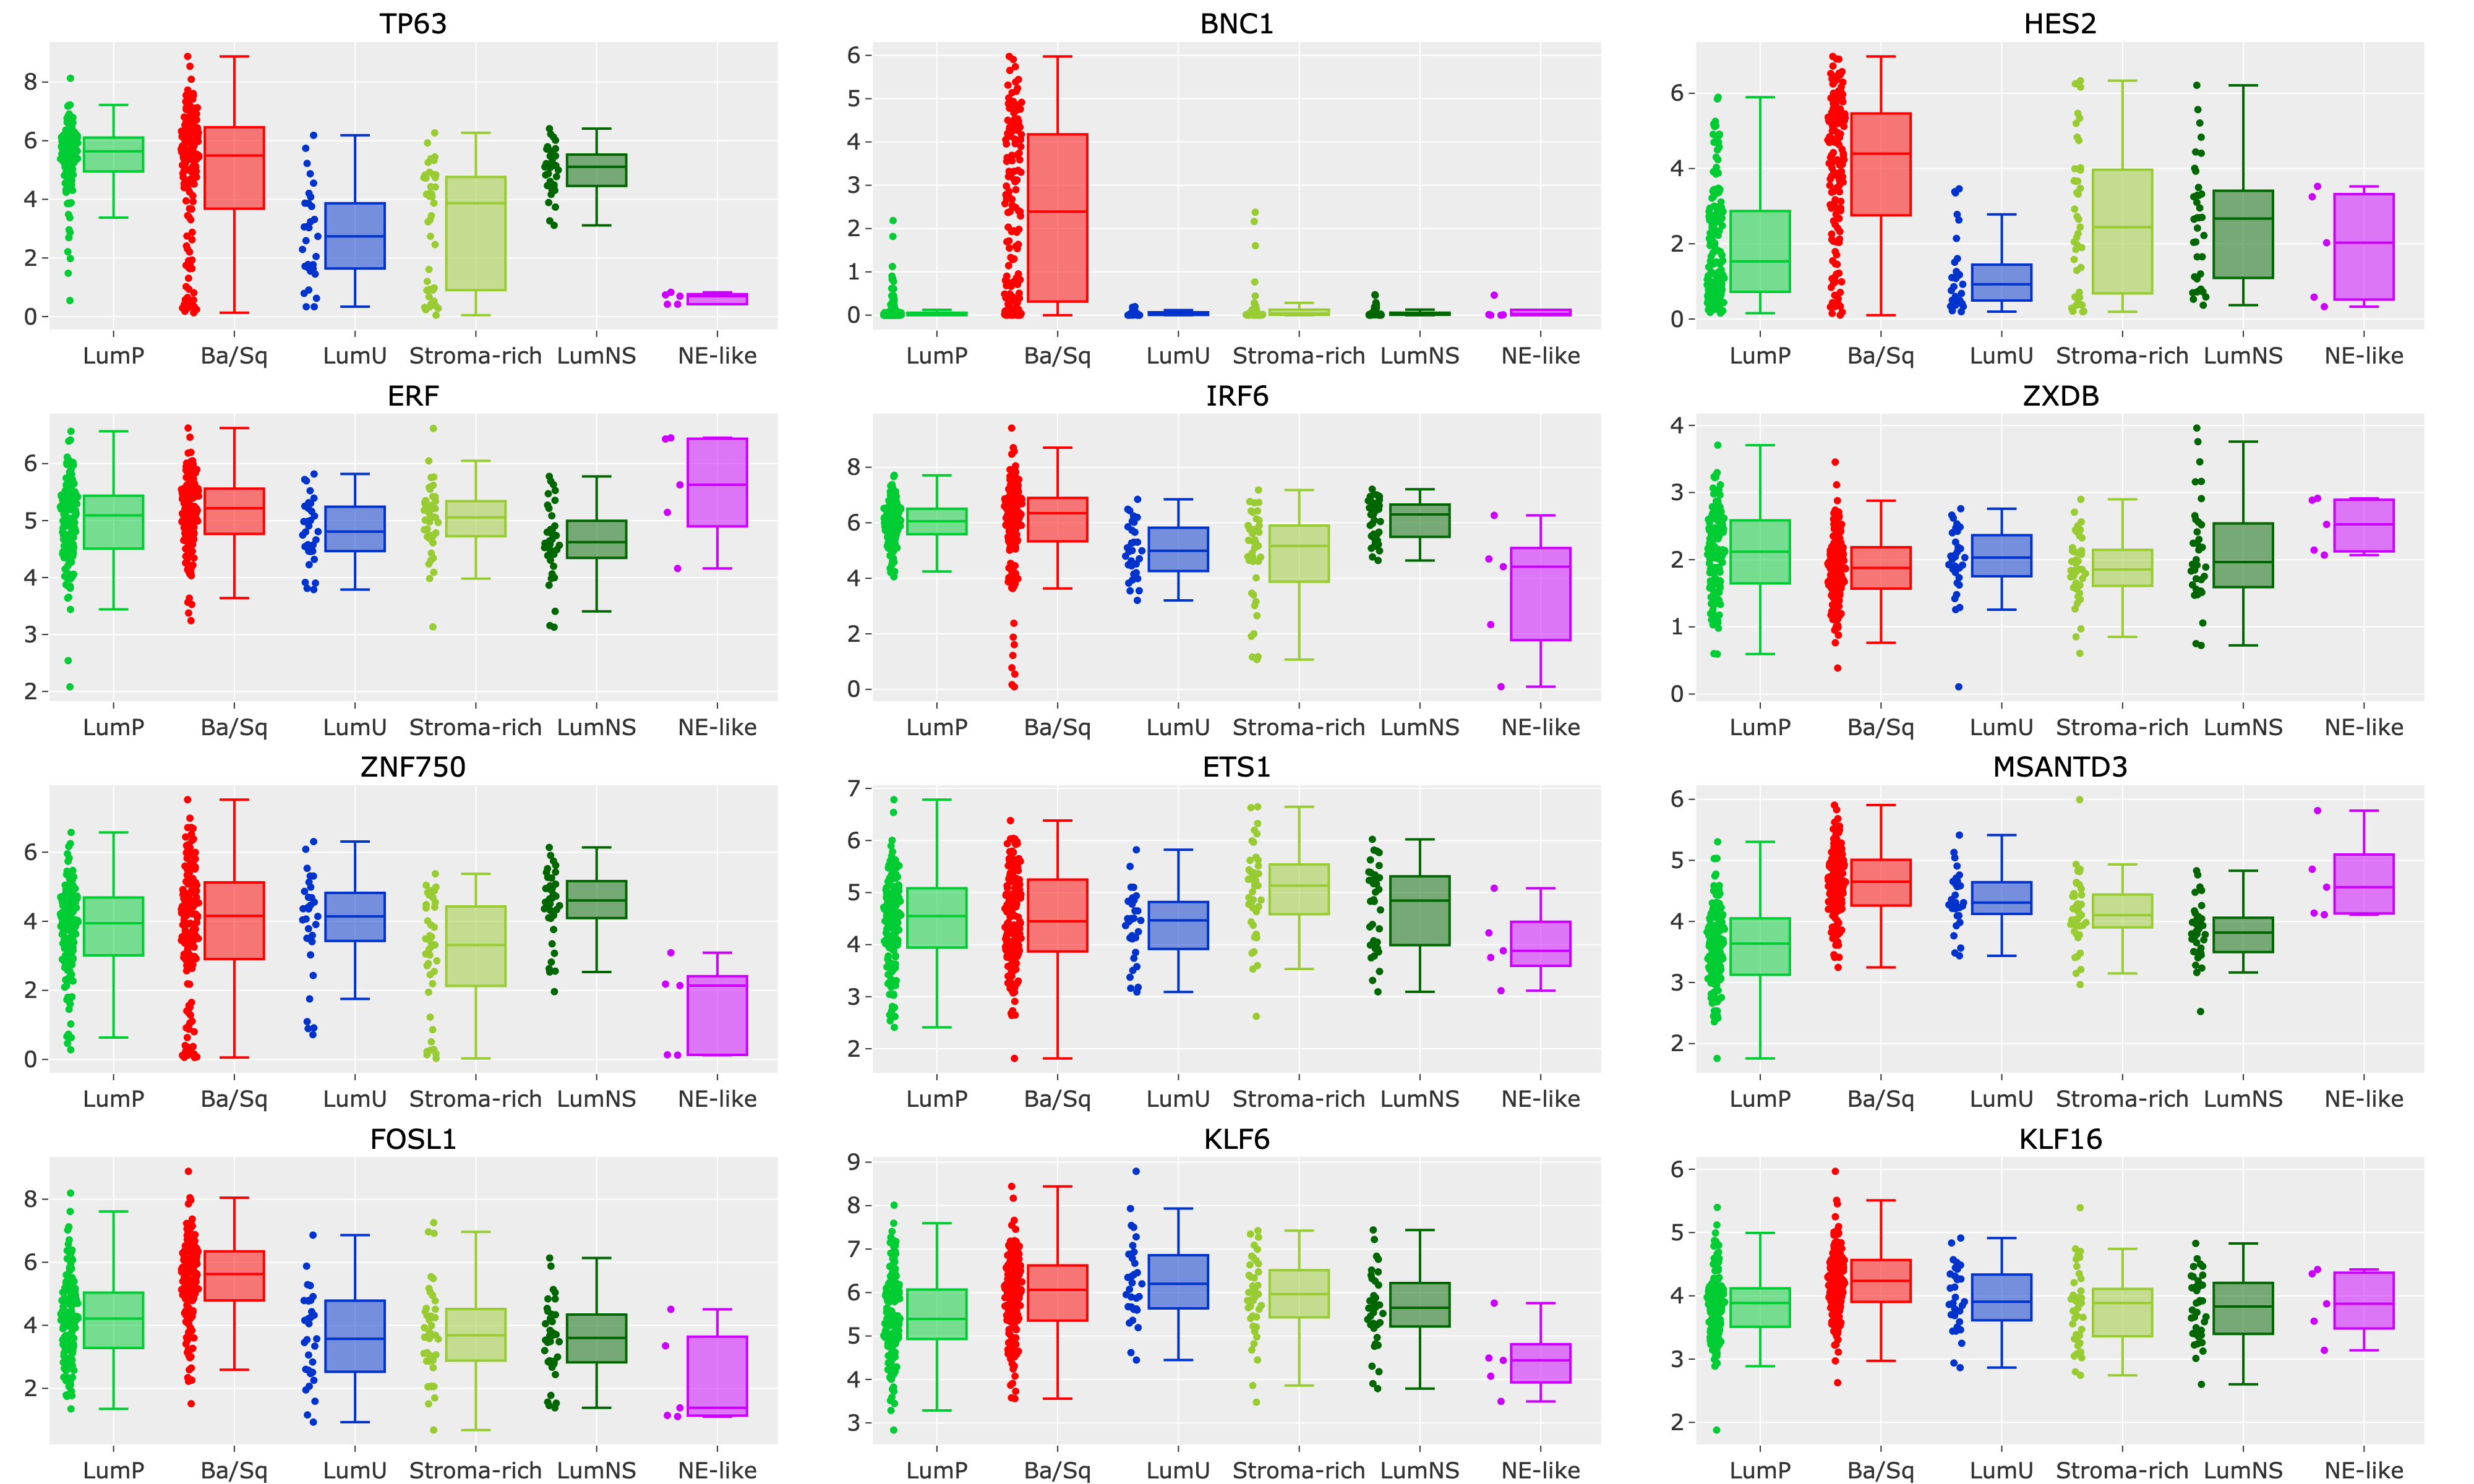
\includegraphics[width=0.49\textheight,keepaspectratio]{Sections/Network_I/Resources/selective_pruning/log2_consensus_basal.png}
%     \caption{Consensus}
%     \label{fig:N_I:box_basal_consensus}
%   \end{subfigure}
%     \begin{subfigure}[!t]{0.49\textwidth}
%      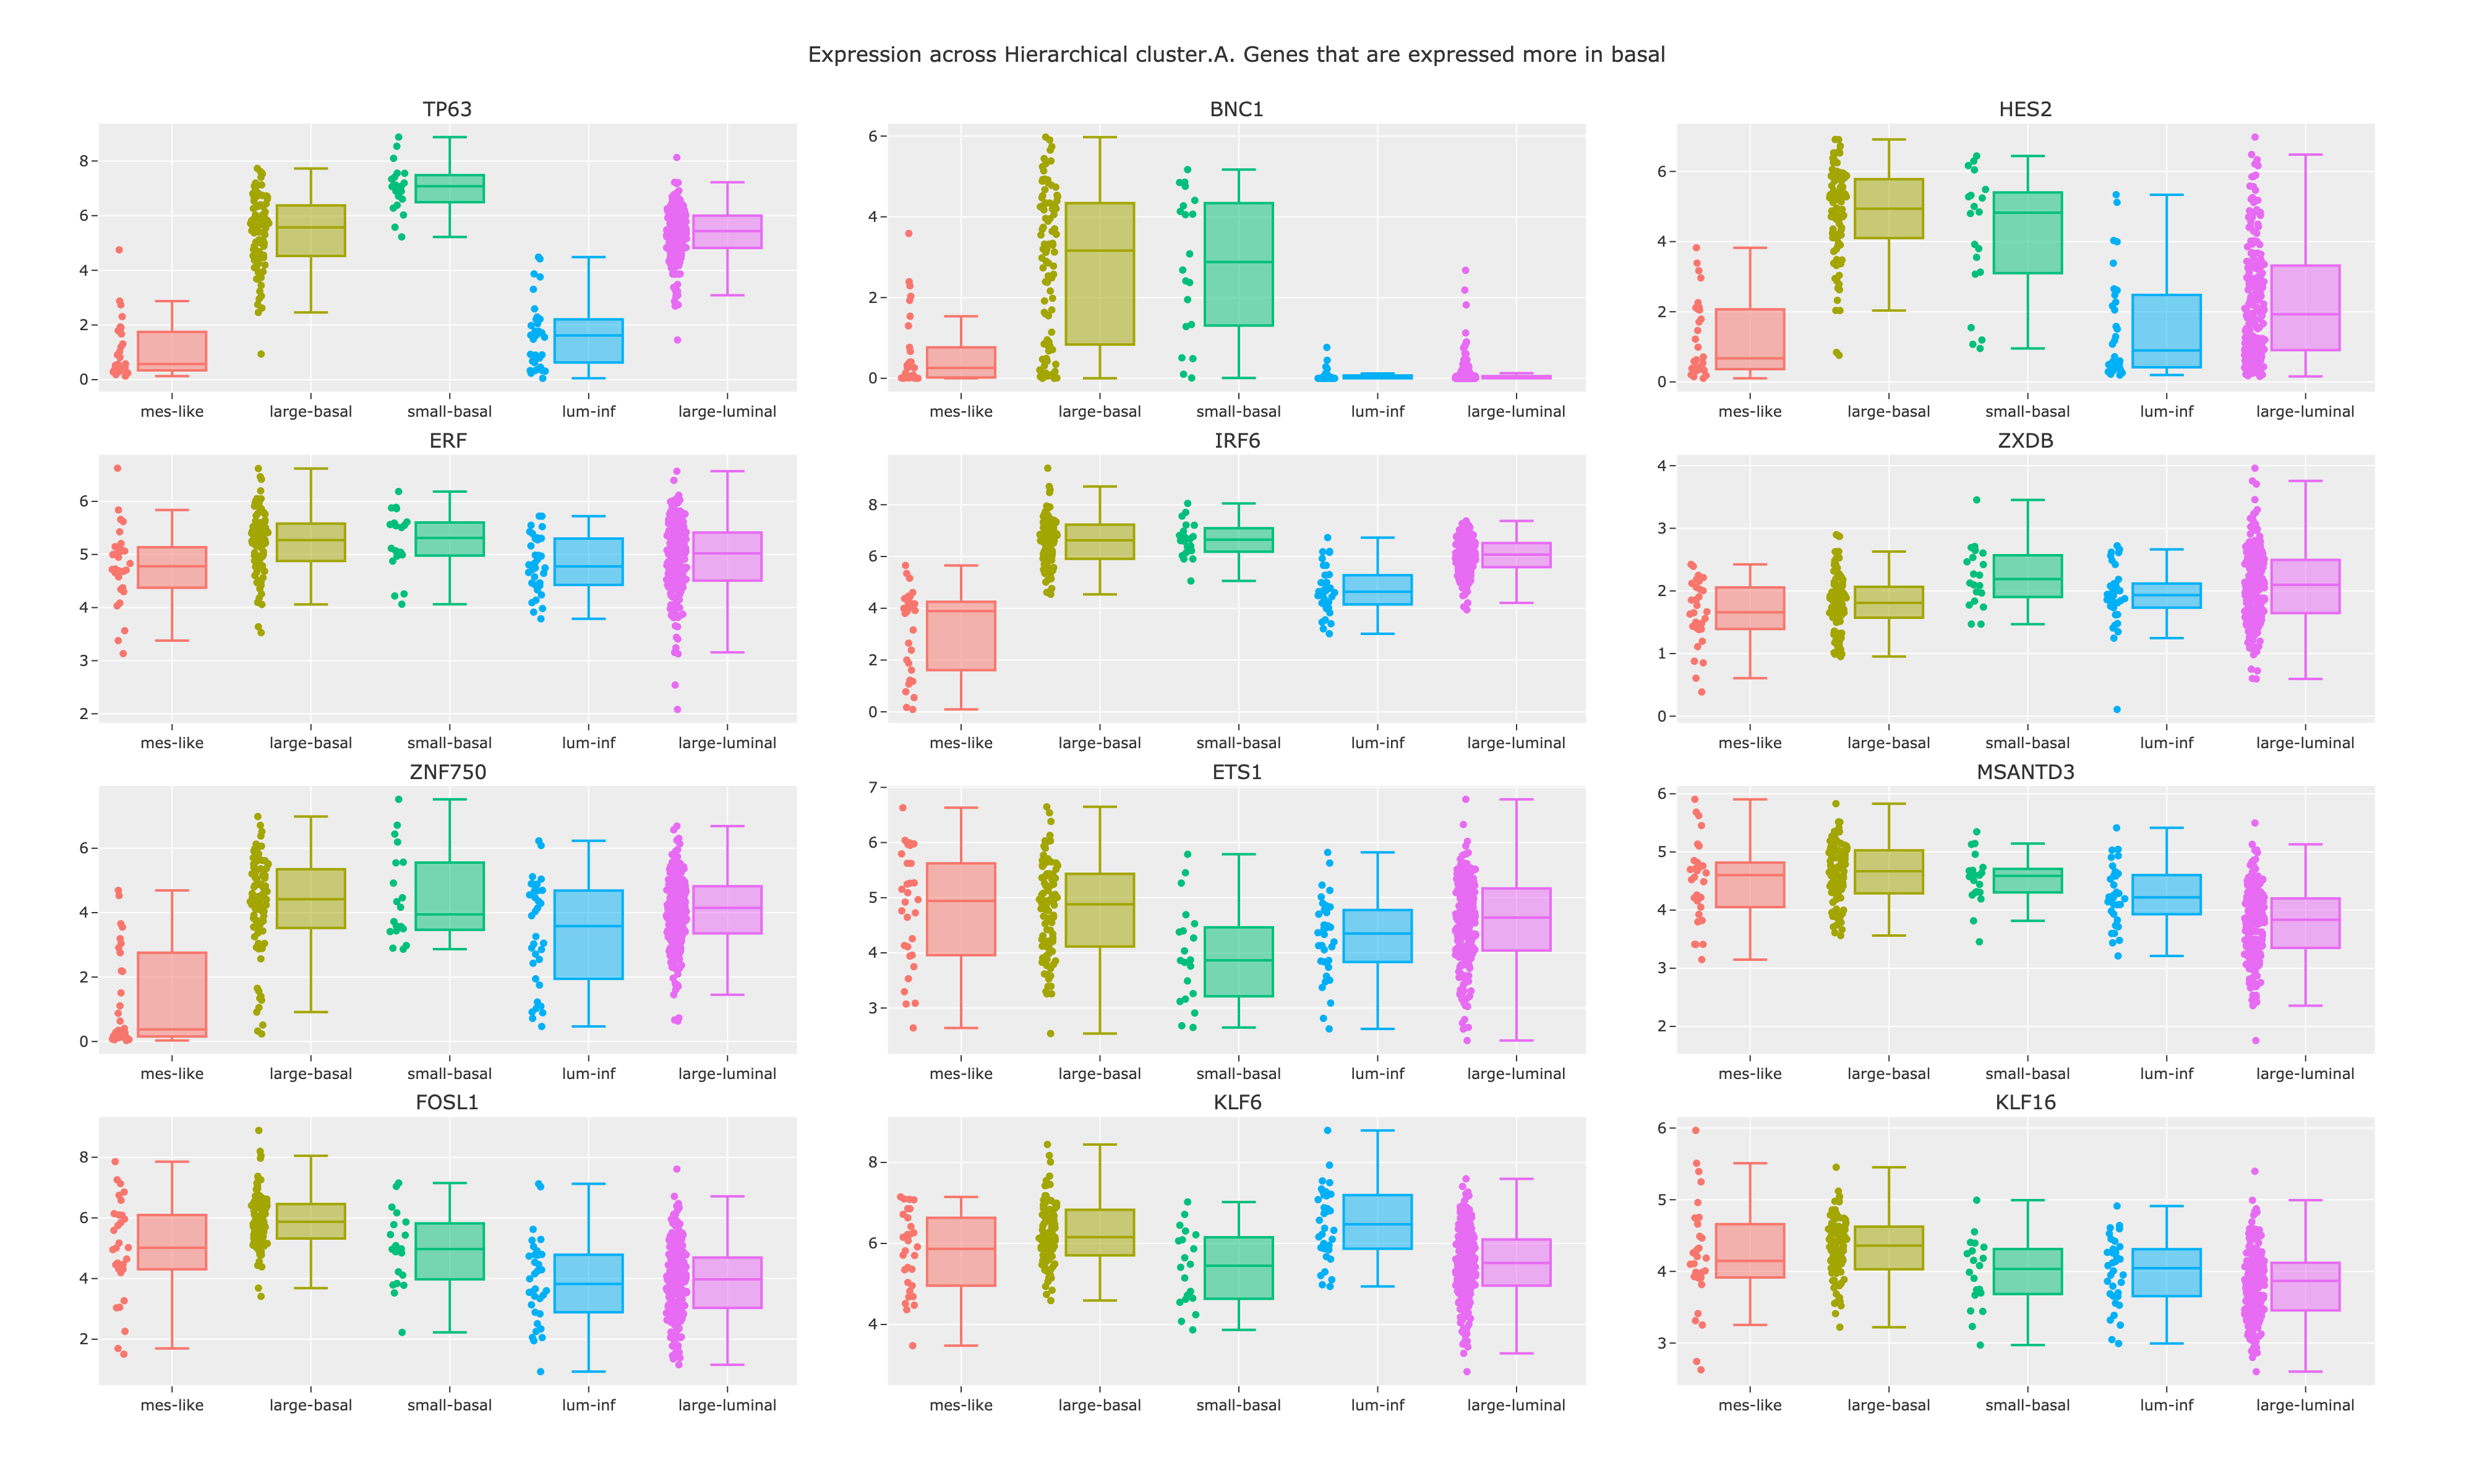
\includegraphics[width=0.49\textheight,keepaspectratio]{Sections/Network_I/Resources/selective_pruning/log2_dendrogram_basla.png}
%       \caption{Basal from hierarchical clustering}
%       \label{fig:N_I:box_basal_dendrogram}
%   \end{subfigure}
%   \caption{Global caption}
% \end{sidewaysfigure}


% Luminal Markers
\begin{figure}[H]
    \captionsetup[subfigure]{justification=Centering}
  % consensus
  \begin{subfigure}[!t]{0.49\textwidth}
      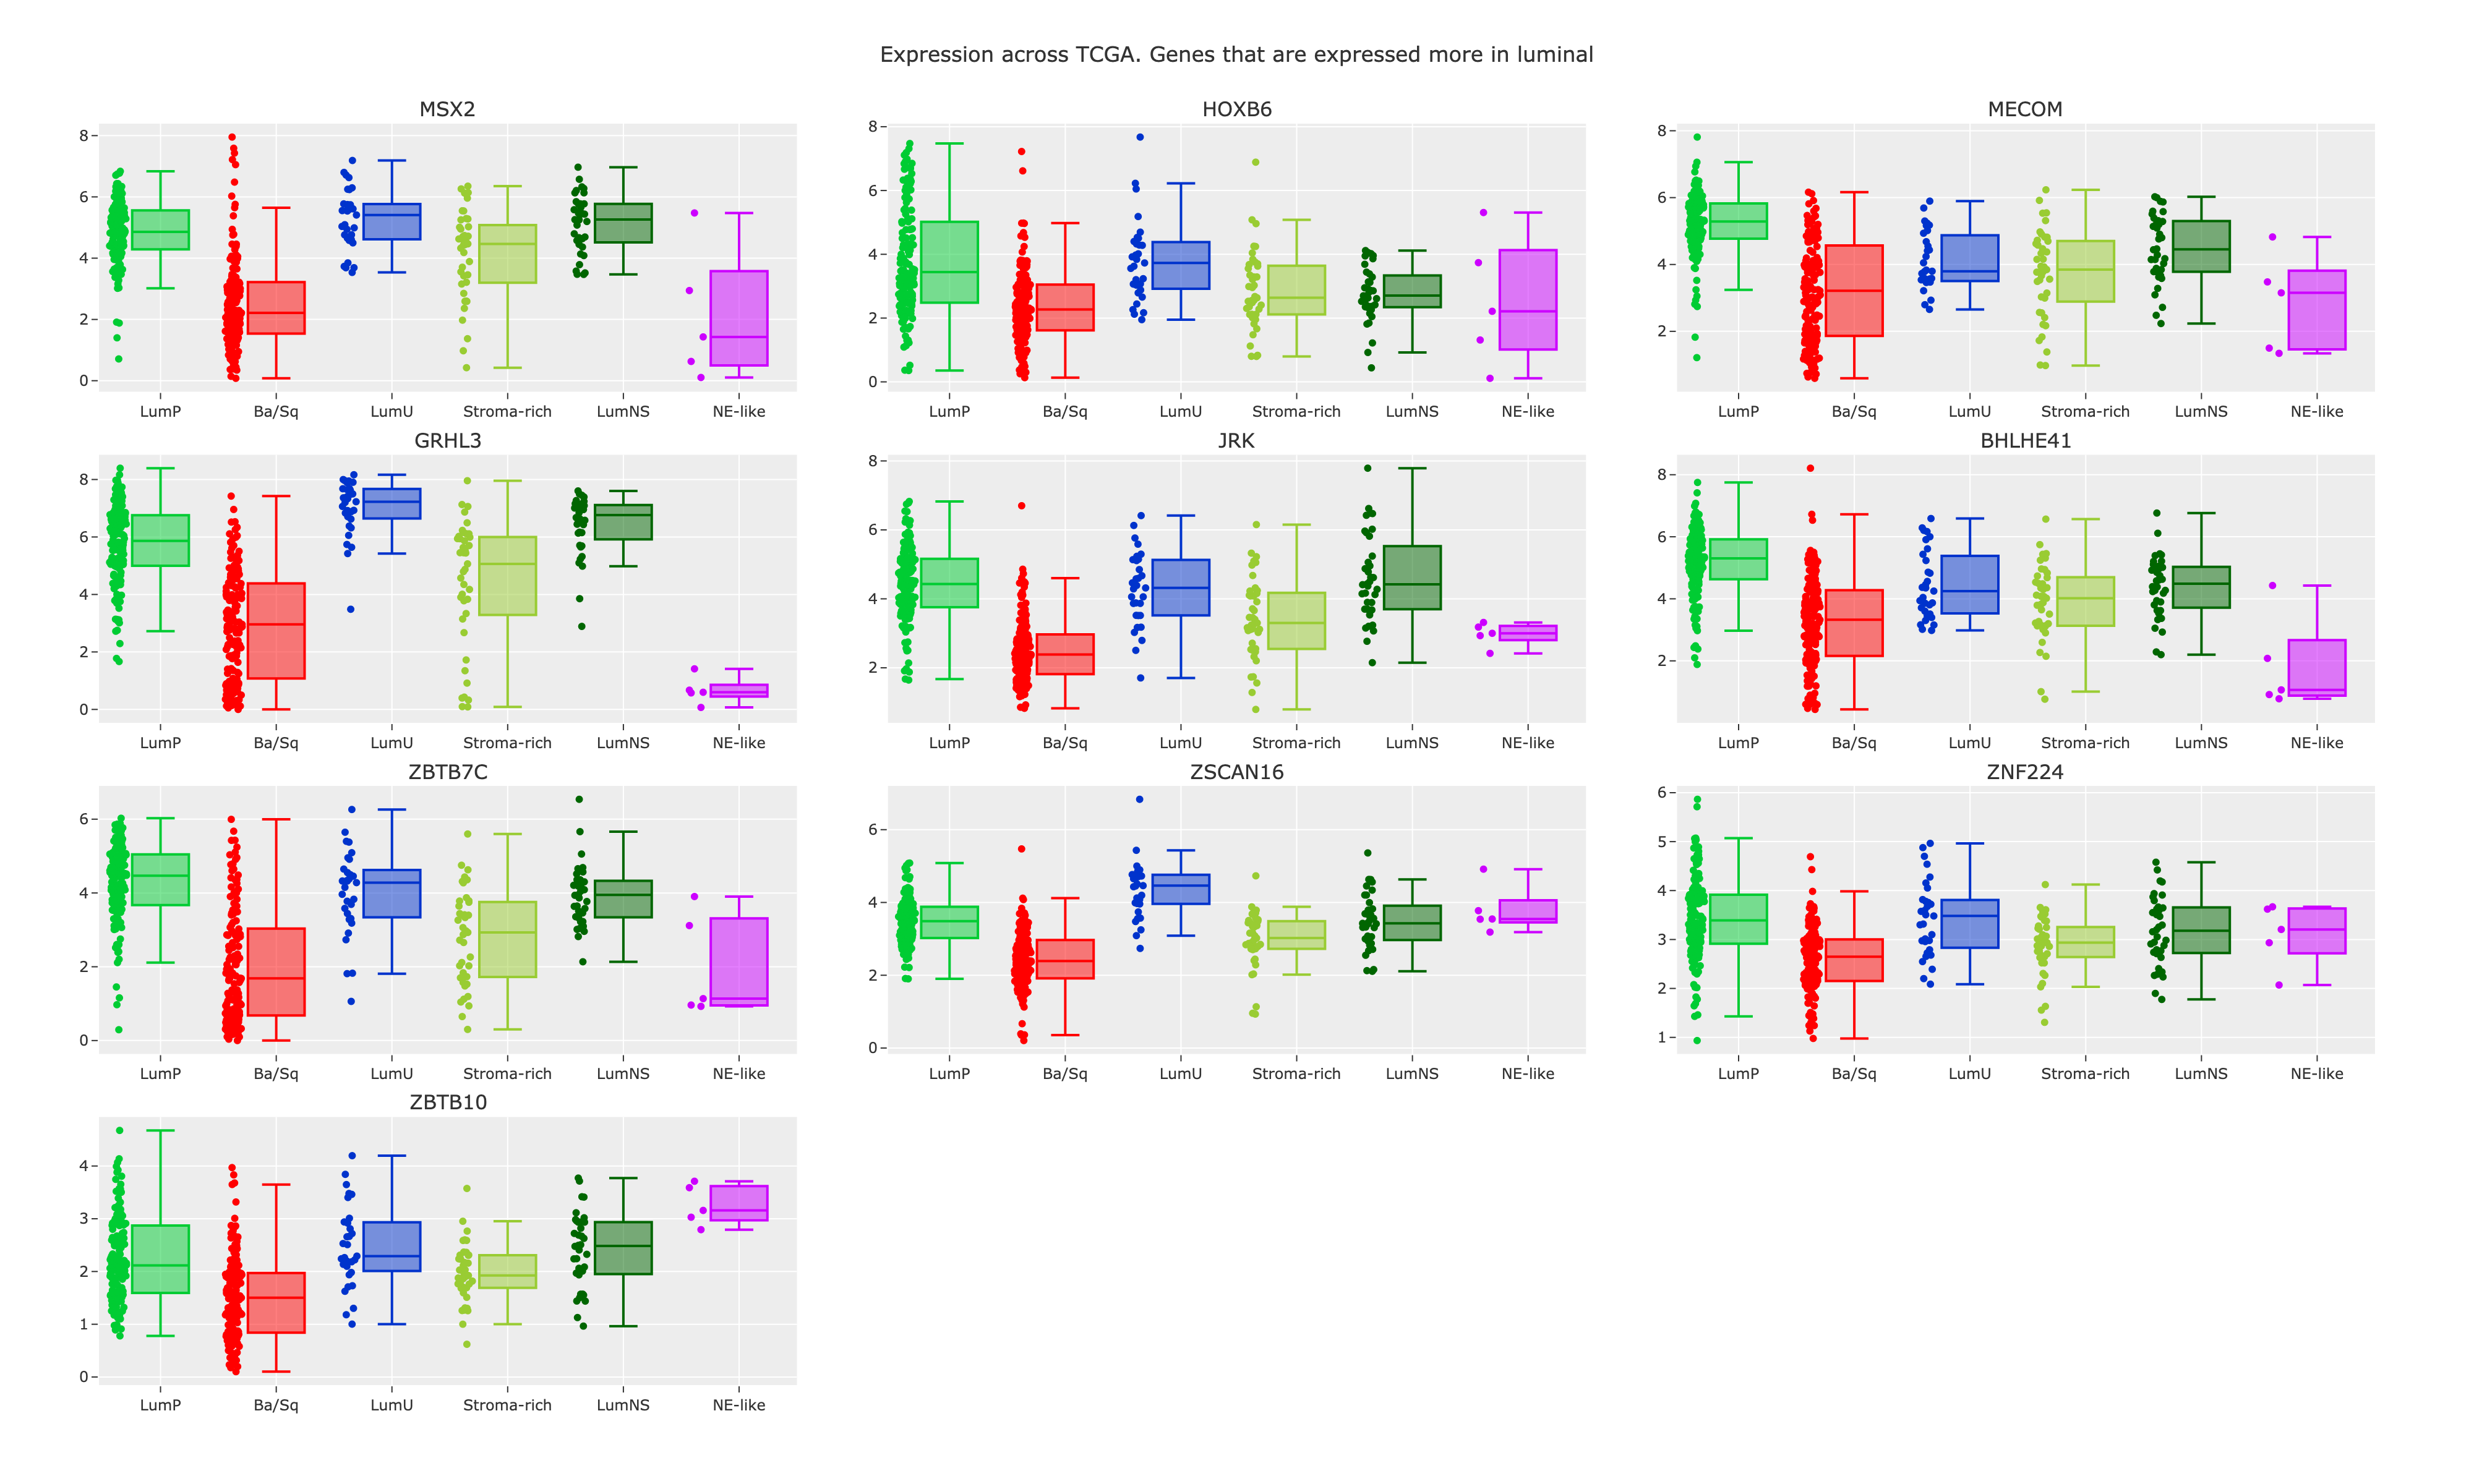
\includegraphics[width=1.0\textwidth,height=1.0\textheight,keepaspectratio]{Sections/Network_I/Resources/selective_pruning/log2_consensus_lum.png}
      \caption{Consensus}
      \label{fig:N_I:box_luminal_consensus}
  \end{subfigure}
  \begin{subfigure}[!t]{0.49\textwidth}
      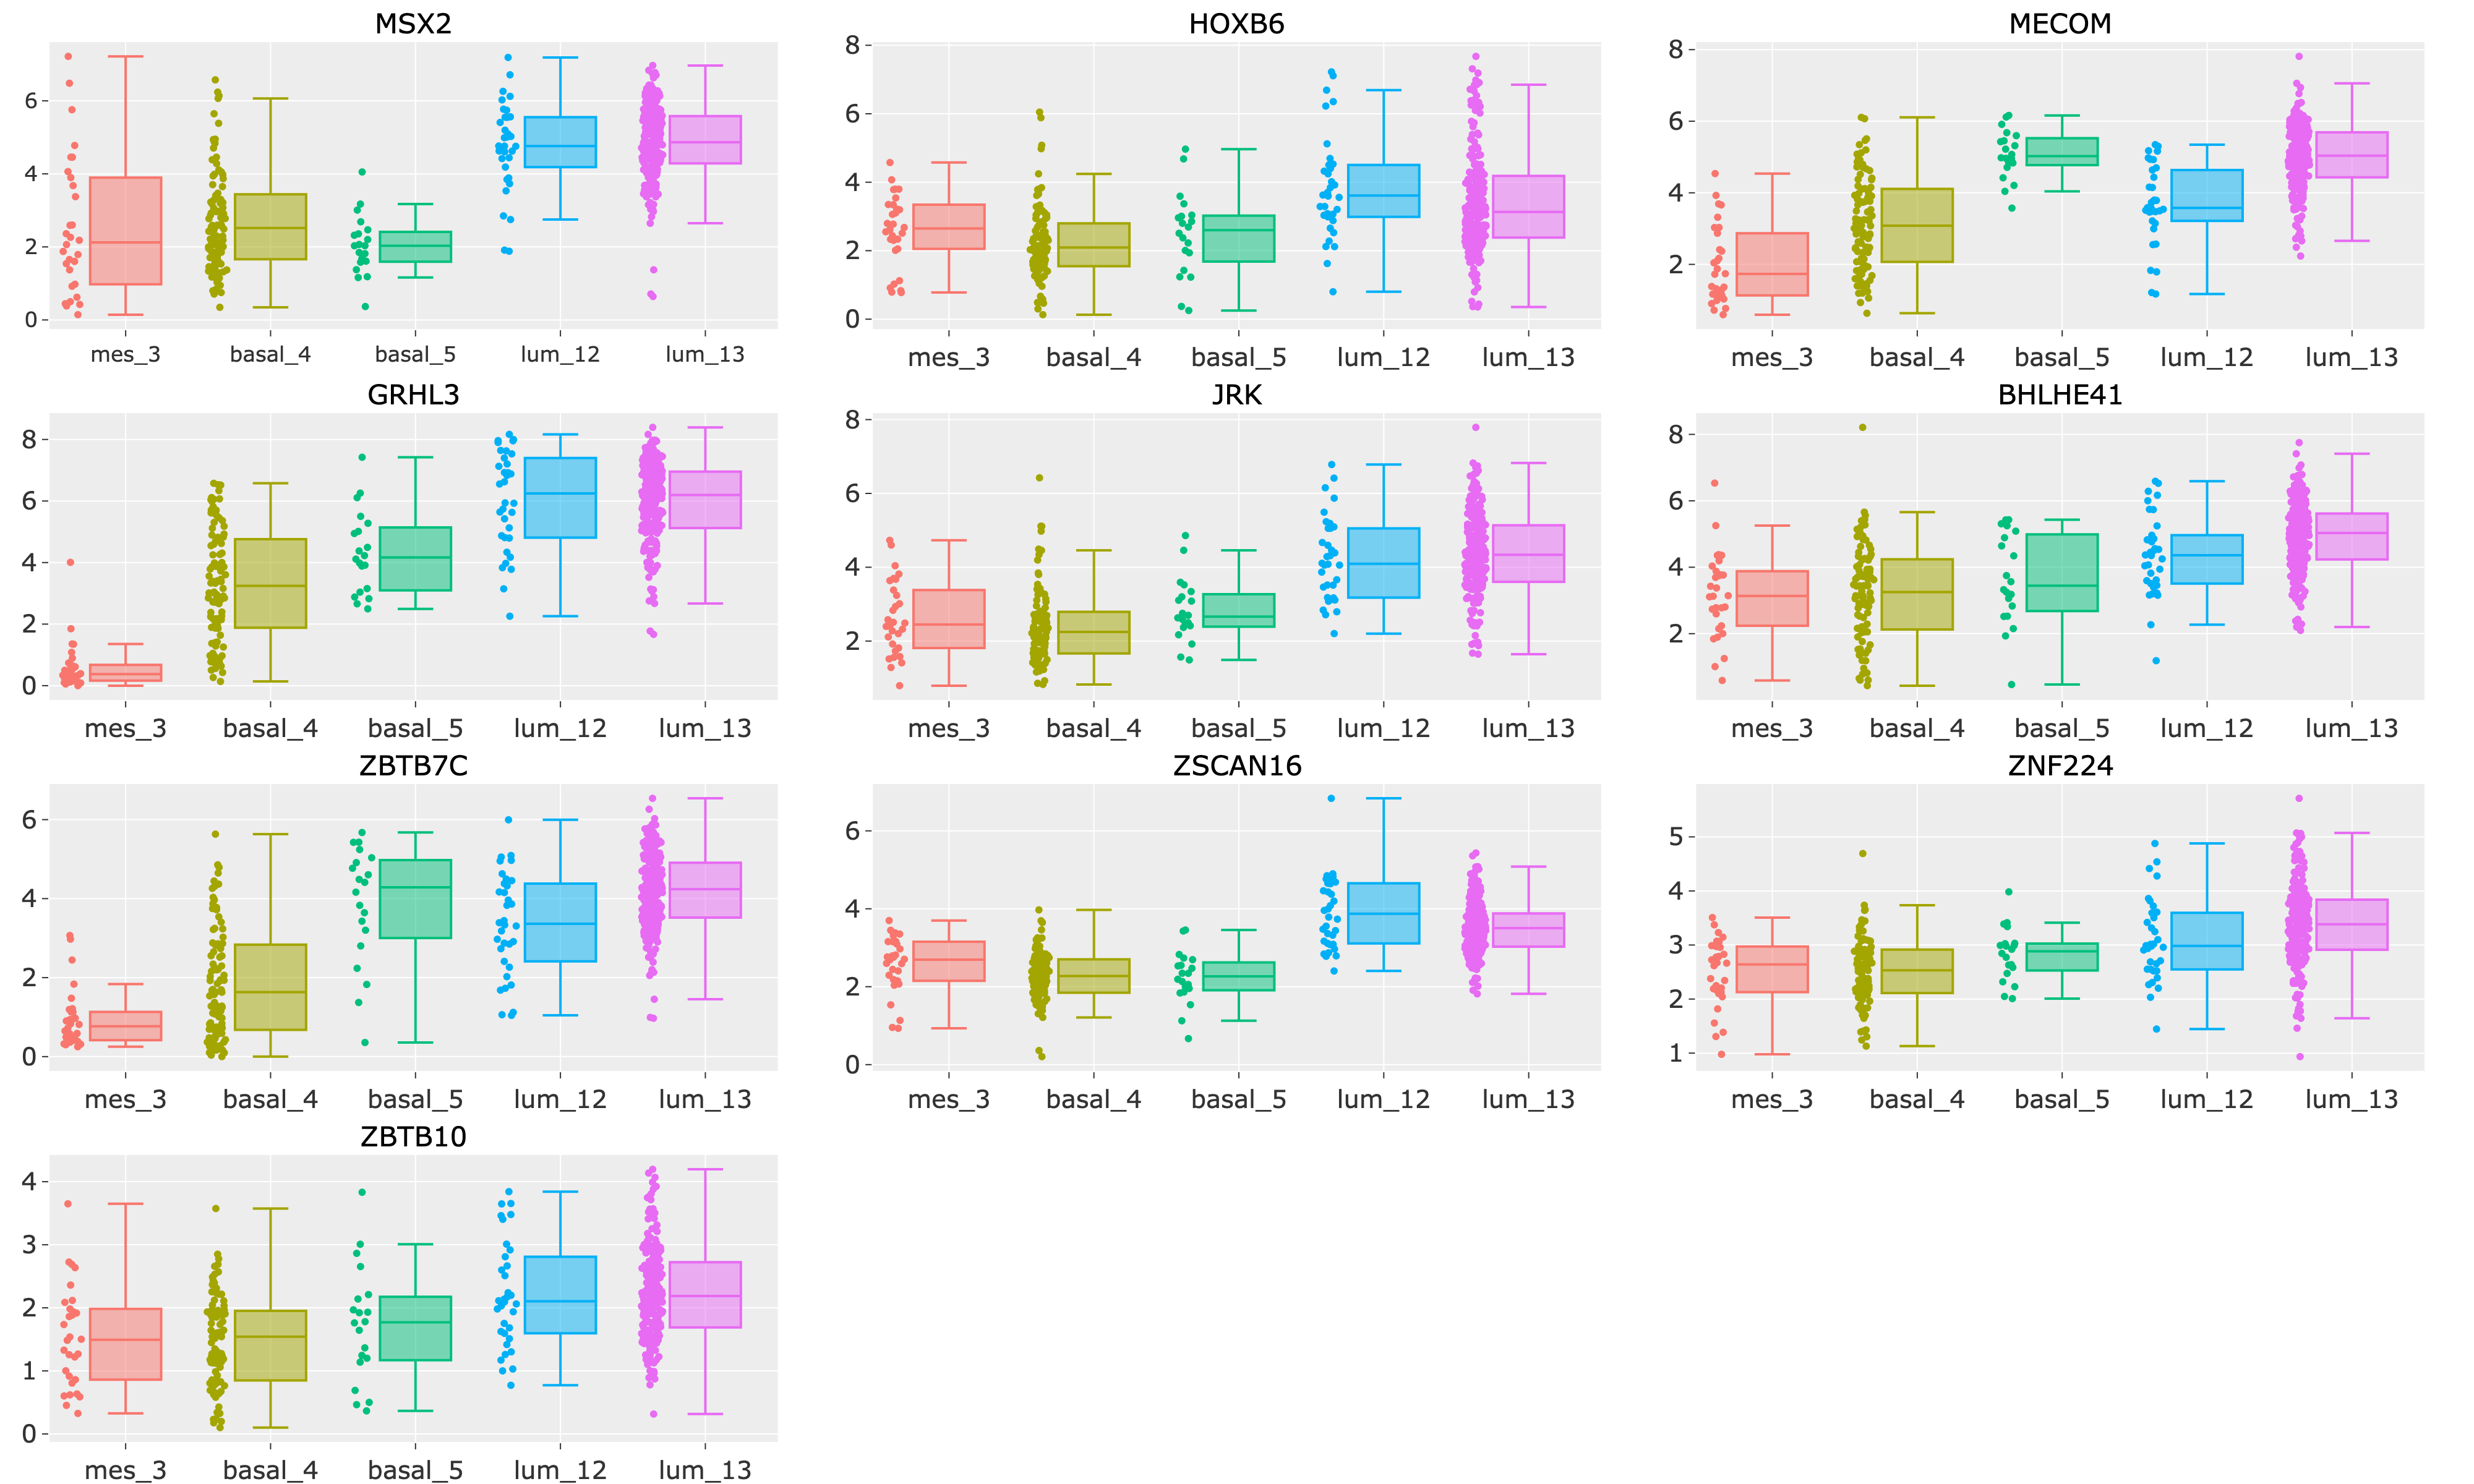
\includegraphics[width=1.0\textwidth,height=1.0\textheight,keepaspectratio]{Sections/Network_I/Resources/selective_pruning/log2_dendrogram_lum.png}
      \caption{Basal}
      \label{fig:N_I:box_luminal_dendrogram}
  \end{subfigure}
  \caption{Box plots showing the $log2(TPM+1)$ of the \textbf{luminal markers} over the consensus and groups derived from the hierarchical clustering applied in this chapter.}
  \label{fig:N_I:box_luminal}
\end{figure}

\subsection{Returning to the network}

% Network stats
To leverage visualising aspect of the network, the basal/luminal markers were then searched in the experiment 5K genes network generated using no weight modifiers (standard), minimum 3 edges per genes and 6 for the TFs, and to which the Stochastic Block Model (SBM) was applied. Neither of the markers, basal/luminal or for differentiated, were not grouped in a single or 2-3 communities, but rather spread across several.

% Neighbours 
When filtering the network to display the neighbours of a  gene from the basal/luminal markers, it is often the case that markers are linked together, meaning that are co-expressed. \Cref{fig:N_I:net_MSX2} shows the sub-graph for \textit{MSX2} in which other markers such as \textit{FOXQ1, ZBTB7C} are linked directly to the gene. \textit{AHR} is also connected to \textit{MSX2}. \textit{AHR} has been extensively studies in the bladder cancer, urothelium and it is highly mutated in the TCGA cohort. It is also studied in more depth in the next chapter \ref{}. In the sub-network for \textit{BNC1} , \cref{fig:N_I:net_BNC1}, there are less known genes but \textit{CDH3} is a basal marker \citet{Dadhania2016-cb} and \textit{CAV1, CAV2}. 

It is worth noting that both genes, have considerable more than 6 neighbours. This suggests that there are many genes that have either \textit{BNC1} or \textit{MSX2} in their top correlated values. The kind of visualisation in \cref{fig:N_I:net_neighbours} is useful to narrow down the search for targets and potential co-expressed genes.

\begin{figure}[H]
    \captionsetup[subfigure]{justification=Centering}
\centering
\begin{subfigure}[!t]{0.49\textwidth}
    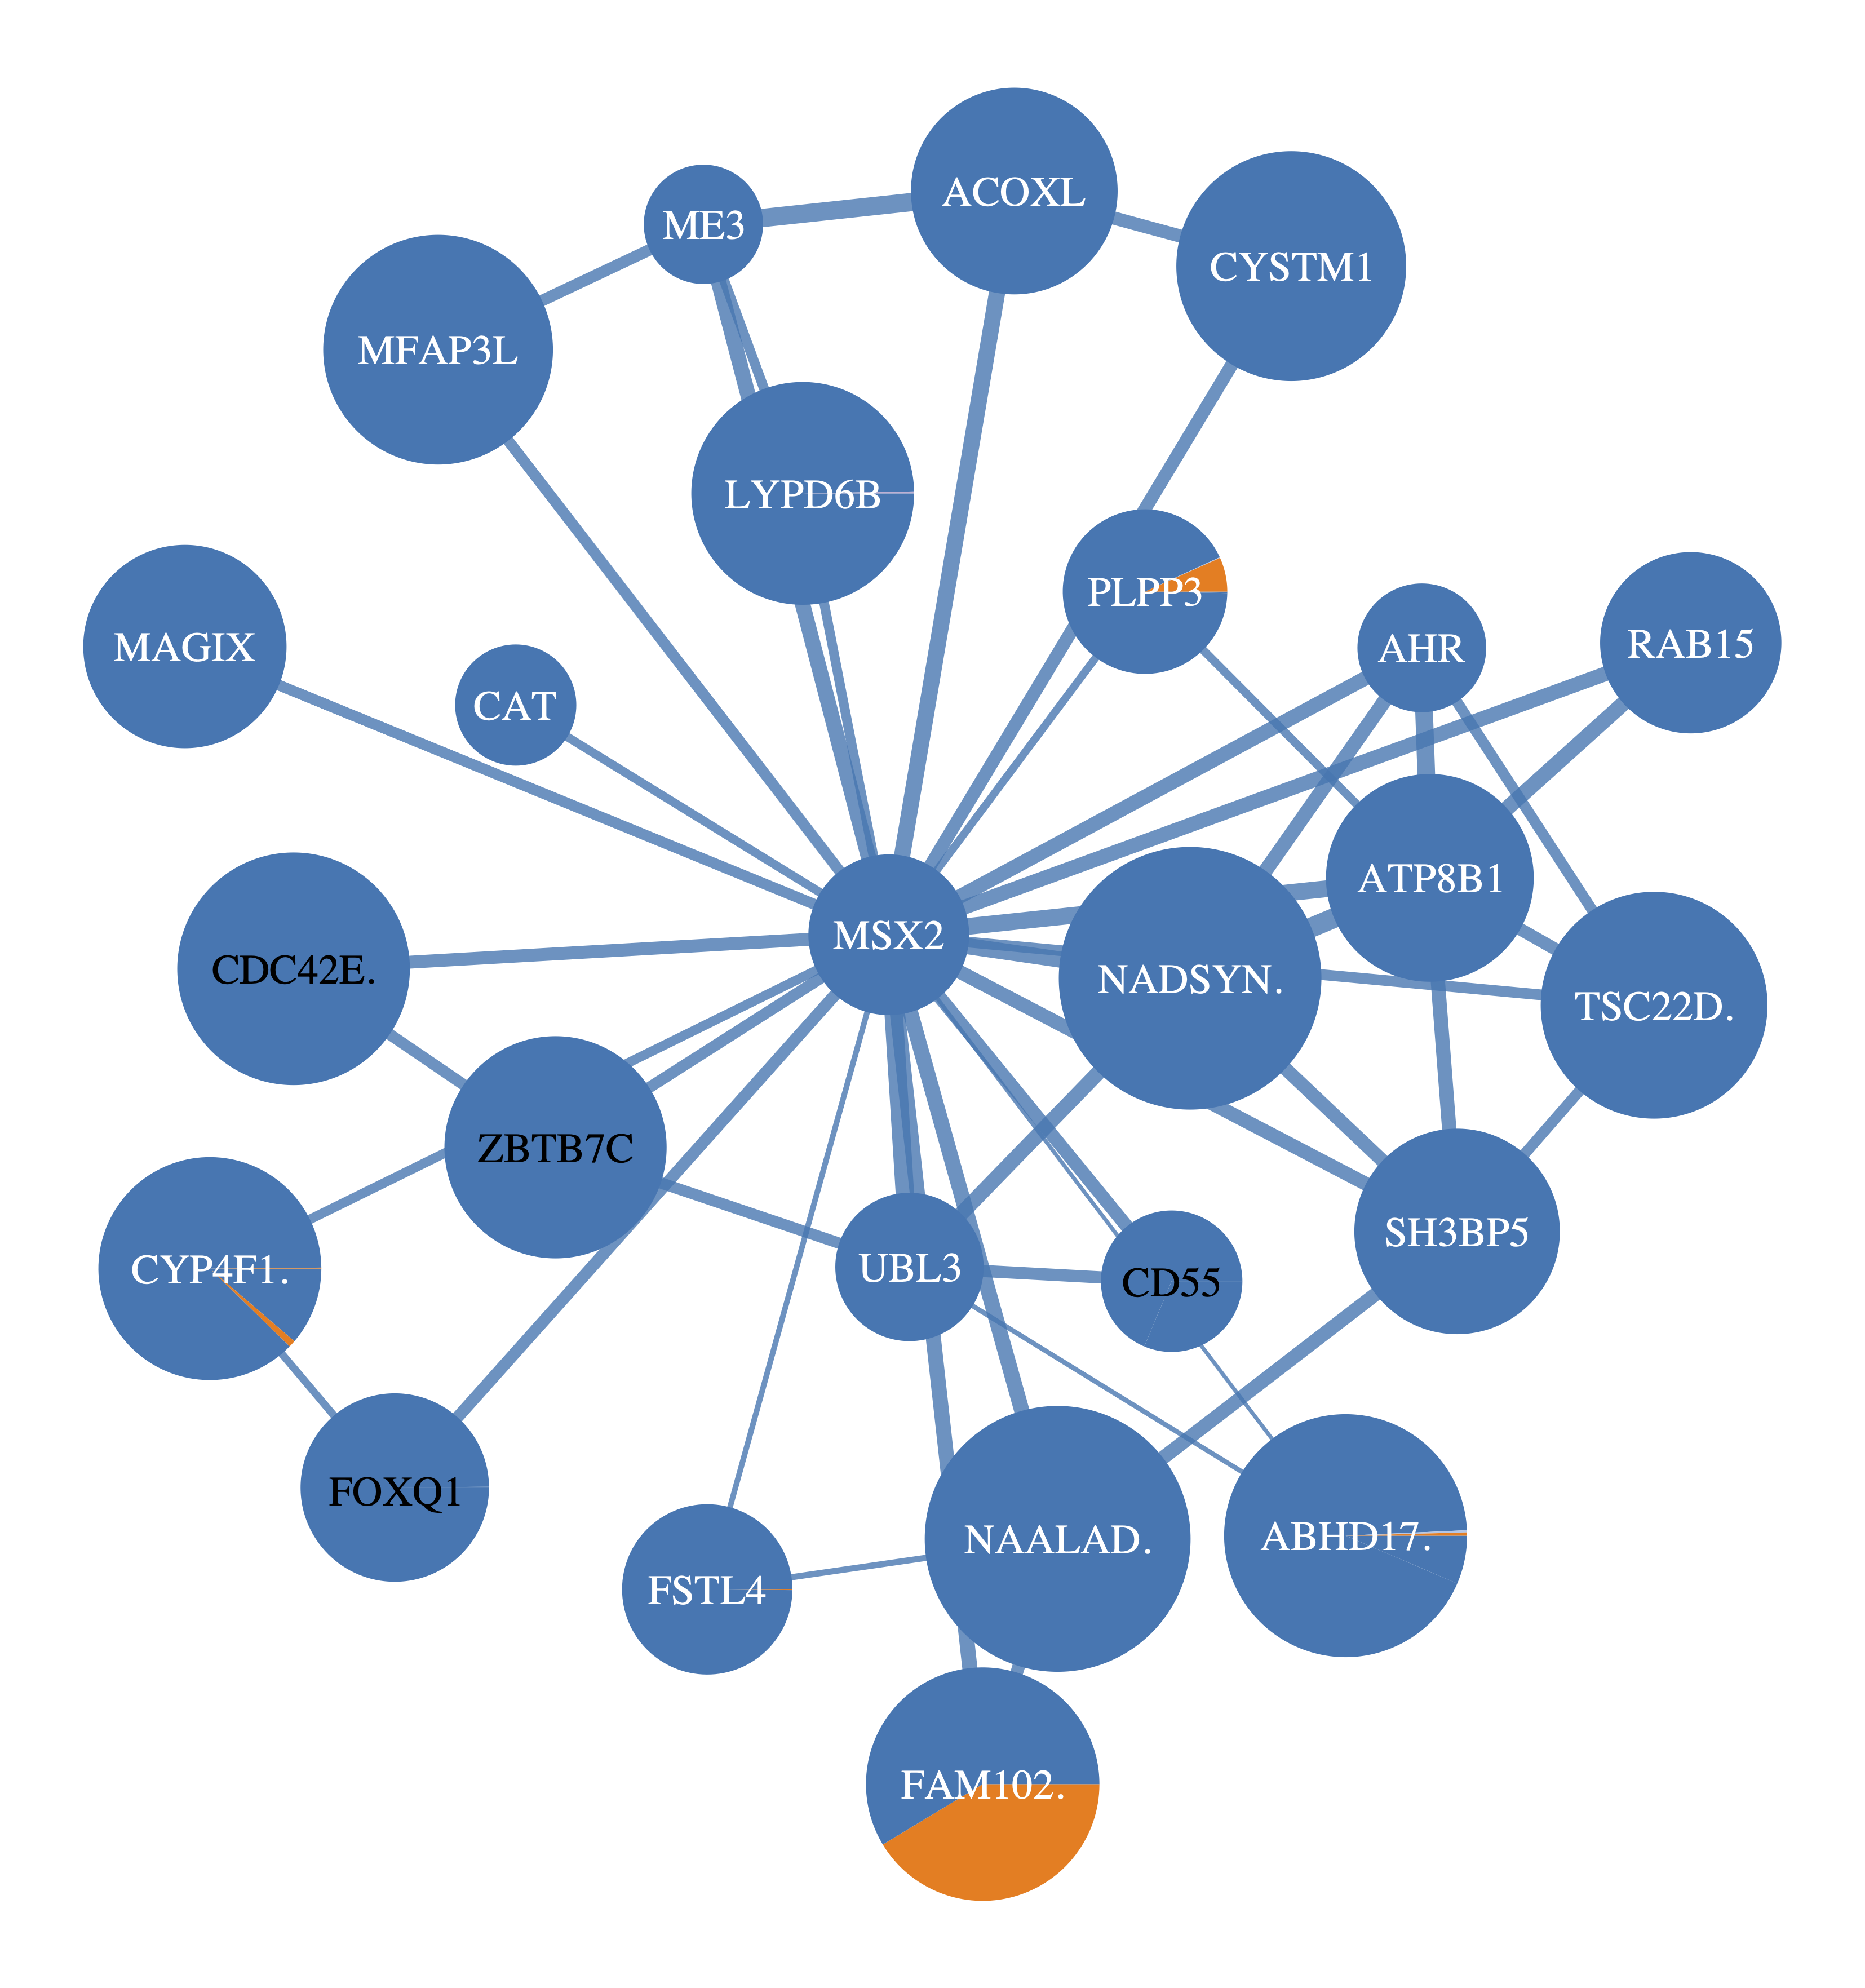
\includegraphics[width=1.0\textwidth,height=1.0\textheight,keepaspectratio]{Sections/Network_I/Resources/selective_pruning/net/net_MSX2.png}
    \caption{\textit{MSX2} (luminal)}
    
    \label{fig:N_I:net_MSX2}
\end{subfigure}
\centering
\begin{subfigure}[!t]{0.49\textwidth}
    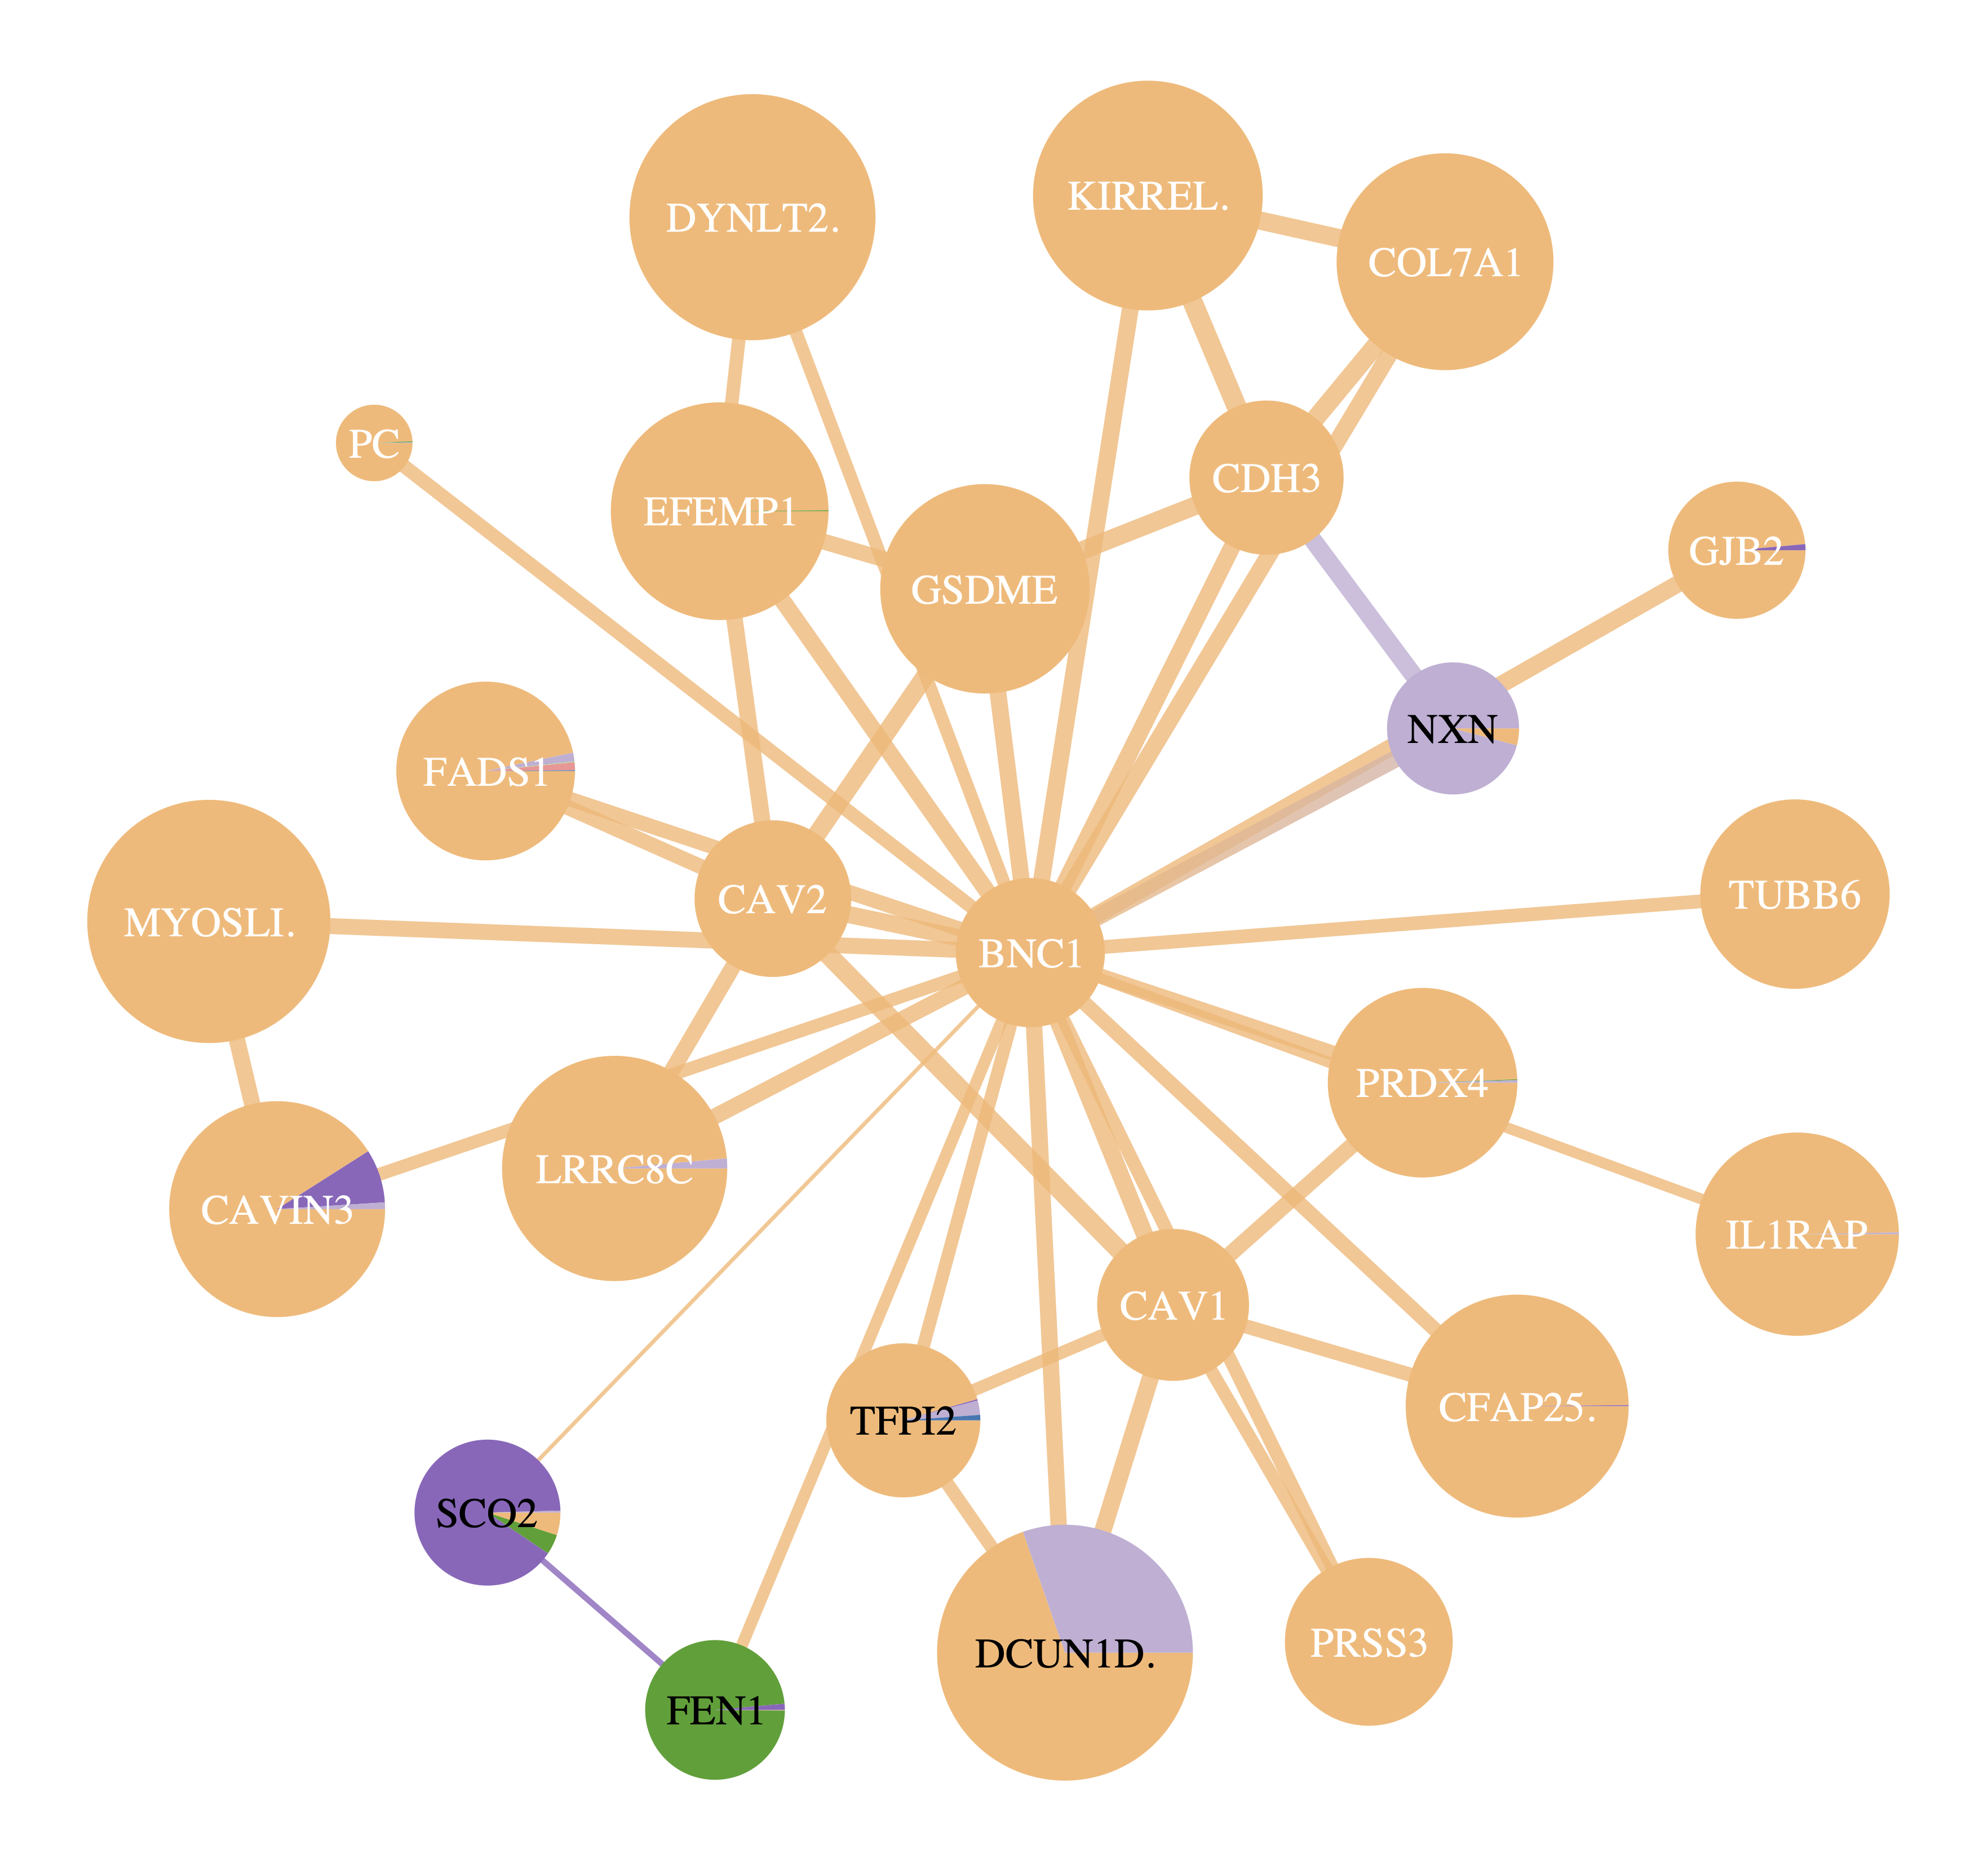
\includegraphics[width=1.0\textwidth,height=1.0\textheight,keepaspectratio]{Sections/Network_I/Resources/selective_pruning/net/net_BNC1.png}
    \caption{\textit{BNC1} (basal)}
    \label{fig:N_I:net_BNC1}
\end{subfigure}

    \caption{The \textit{MSX2} luminal and \textit{BNC1} markers and their neighbours in a standard network (no weight modifier), where a minimum of 6 edges are allowed per TF and the Stochastic Block Model was applied to detect the communities. The size of the nodes is proportional to the degree of the gene and the edge weight to the correlation value.}
    
    \label{fig:N_I:net_neighbours}
\end{figure}


Therefore, the 98 transcription factors and the two lists of Ba/Sq and Luminal markers are validated by research from different groups. The expression of these genes across the MIBC, from both the consensus and the subtypes derived from hierarchical clustering, can be seen in \cref{fig:N_I:box_basal,fig:N_I:box_luminal}. This also serves as an encouragement to explore the other genes not matched by other research, as they may exhibit potential for new biological insights.

